 \documentclass{article}
    \usepackage{amsmath}
    \usepackage[utf8]{inputenc}
    \usepackage[english]{babel}
    \usepackage{color}
    \usepackage{graphicx}
    \usepackage{enumitem}
    \usepackage{incgraph}
    \hyphenpenalty=10000
    \exhyphenpenalty=10000
    % \usepackage[T1]{fontenc}
    % \usepackage{geometry}
    \usepackage[top = 2cm, bottom = 2cm]{geometry}
    
    \usepackage[familydefault,light]{Chivo} 
    \usepackage[T1]{fontenc}
    
    \setlength{\parindent}{4em}
    \setlength{\parskip}{2em}
\renewcommand{\baselinestretch}{1.5}
    \usepackage{graphicx}
    
    \usepackage{listings}
    \usepackage{color}
    
    \definecolor{dkgreen}{rgb}{0,0.6,0}
    \definecolor{gray}{rgb}{0.5,0.5,0.5}
    \definecolor{mauve}{rgb}{0.58,0,0.82}
    
    \lstset{frame=tb,
      language=ocaml,
      aboveskip=3mm,
      belowskip=3mm,
      showstringspaces=false,
      columns=flexible,
      basicstyle={\small\ttfamily},
      numbers=none,
      numberstyle=\tiny\color{gray},
      keywordstyle=\color{blue},
      commentstyle=\color{dkgreen},
      stringstyle=\color{mauve},
      breaklines=true,
      breakatwhitespace=true,
      tabsize=3
    }
    
    \title{COL 783 \\ Assignment 4}
    \author{Rajbir Malik \\ 2017CS10416}
    
    \begin{document}
    
    \maketitle

%  Starting page
% -------------------------------------------------------
% -------------------------------------------------------
    \begin{center}
    \Large{\underline{\textbf{Robust Form Processing}}}
    \end{center}
    \subsection*{Overview}
    The assignment required us to process some forms in different natural settings, and trying to extract meaningful information from the forms.\\
    Being much open ended, we had the opportunity to try various procedures to get the task done. I was, after many attempts, able to come up with a "mostly" automated process to get the required information.\\ I have presented this approach and explained the procedure in the upcoming report. I've also discussed another approach that was reasonable to some scale, but couldn't be scaled, by me, to the desired level.
% -------------------------------------------------------
% -------------------------------------------------------
% Topic I
    \pagebreak
    \subsection*{Image Alignment}
% -------------------------------------------------------
    I worked upon the lines of a standard form scanner, to get all the input images aligned correctly.\\
    Having created a template-default form, I used it as reference to get the ideal warp-perspective for the input image, with the help of descriptor-matching.\\
    The exact pseudo-code for the same has been described below...\\
    \begin{lstlisting}
def image_alignment(_input_image, _template):
    - Create ORB Descriptor
    - Get Key-Points and Descriptors
    - Match the features
    - Filter the matches, to get the ideal ones for mapping
    - Using keypoints, discover ideal homography
    - Use the homography, and warp the input image
    - Return the warped image
    \end{lstlisting}
\textbf{Results}\\
    The results for alignment procedure were quite-impressive, achieveing as good as 99\% accuracy for \texttt{printouts} and \texttt{scanned} and reasonable results for \texttt{boooklets}. Perhaps, if I could find ideal templates for booklets as well (which I couldn't), then there too a decent result may have been procured.\\
    Further, I present the results of alignment on all the categories (2 of each kind).\\
\textbf{Another Approach}\\
    I also tried with a much simpler approach earlier, which involved finding the lines using \texttt{Canny-Edge Detector} and then using \texttt{Hough-Transform} to get the angle at which maximum no. of lines appeared.\\ This approached, though naive seemed to work sensibly for \texttt{scanned}-images, but failed badly for both \texttt{printouts} and \texttt{boooklets}. So, I was compelled to drop the idea.
% -------------------------------------------------------
\pagebreak
    \begin{figure}[!htb]
    %
    \minipage{\textwidth}
    \begin{center}
      \includegraphics[scale=.065]{4/.report/_orig/p1.jpg}
      \caption{Printouts_1}
    \end{center}
    \endminipage
    \end{figure}
    \begin{figure}[!htb]
    %
    \minipage{\textwidth}
    \begin{center}
      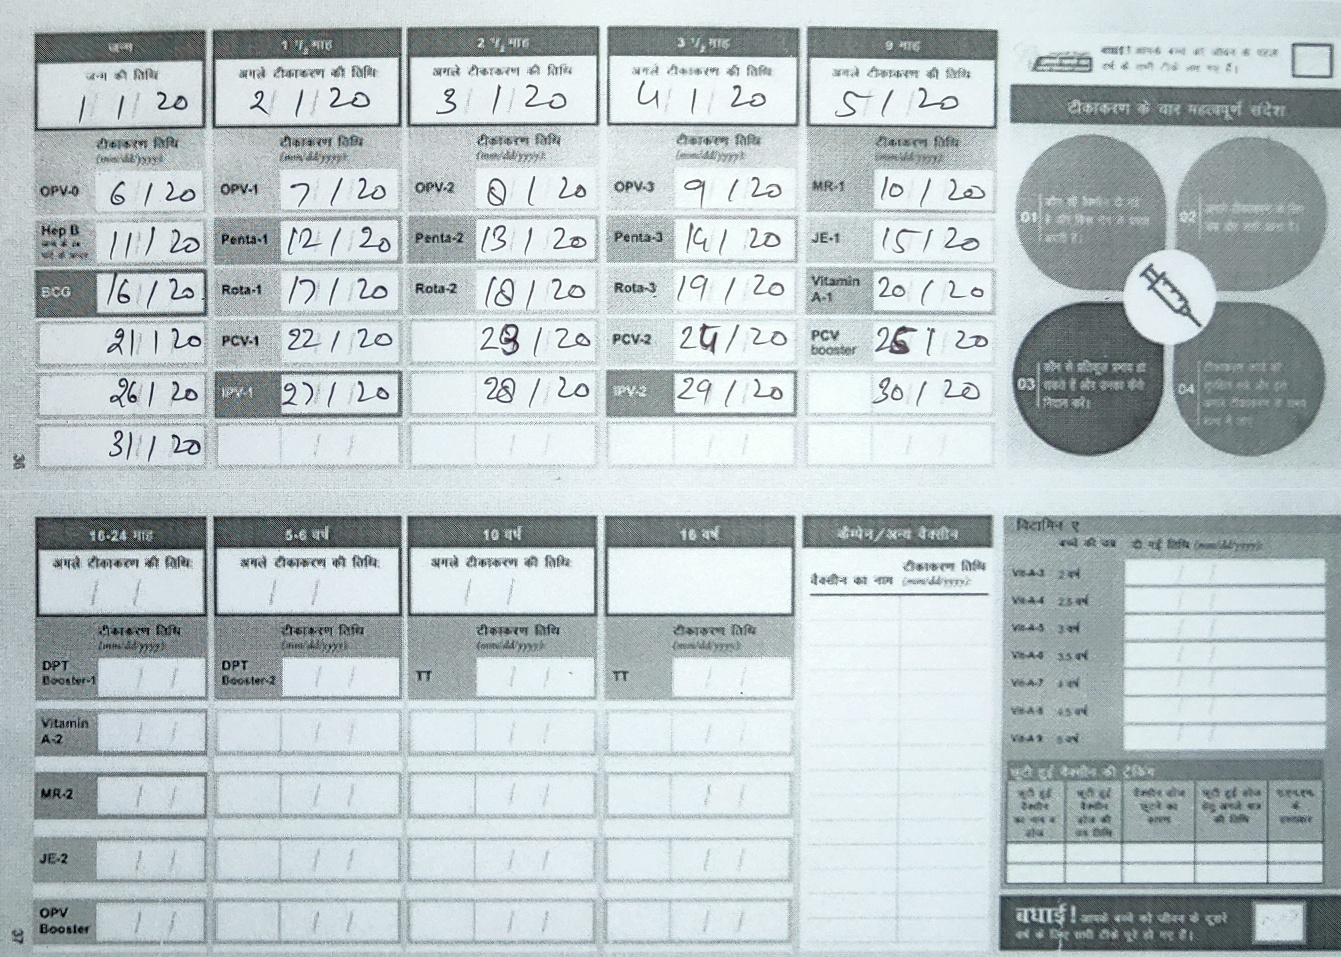
\includegraphics[scale=.2]{4/.report/_aligned/p1.jpg}
      \caption{Aligned}
    \end{center}
    \endminipage
    \end{figure}

% -------------------------------------------------------
\pagebreak
    \begin{figure}[!htb]
    %
    \minipage{\textwidth}
    \begin{center}
      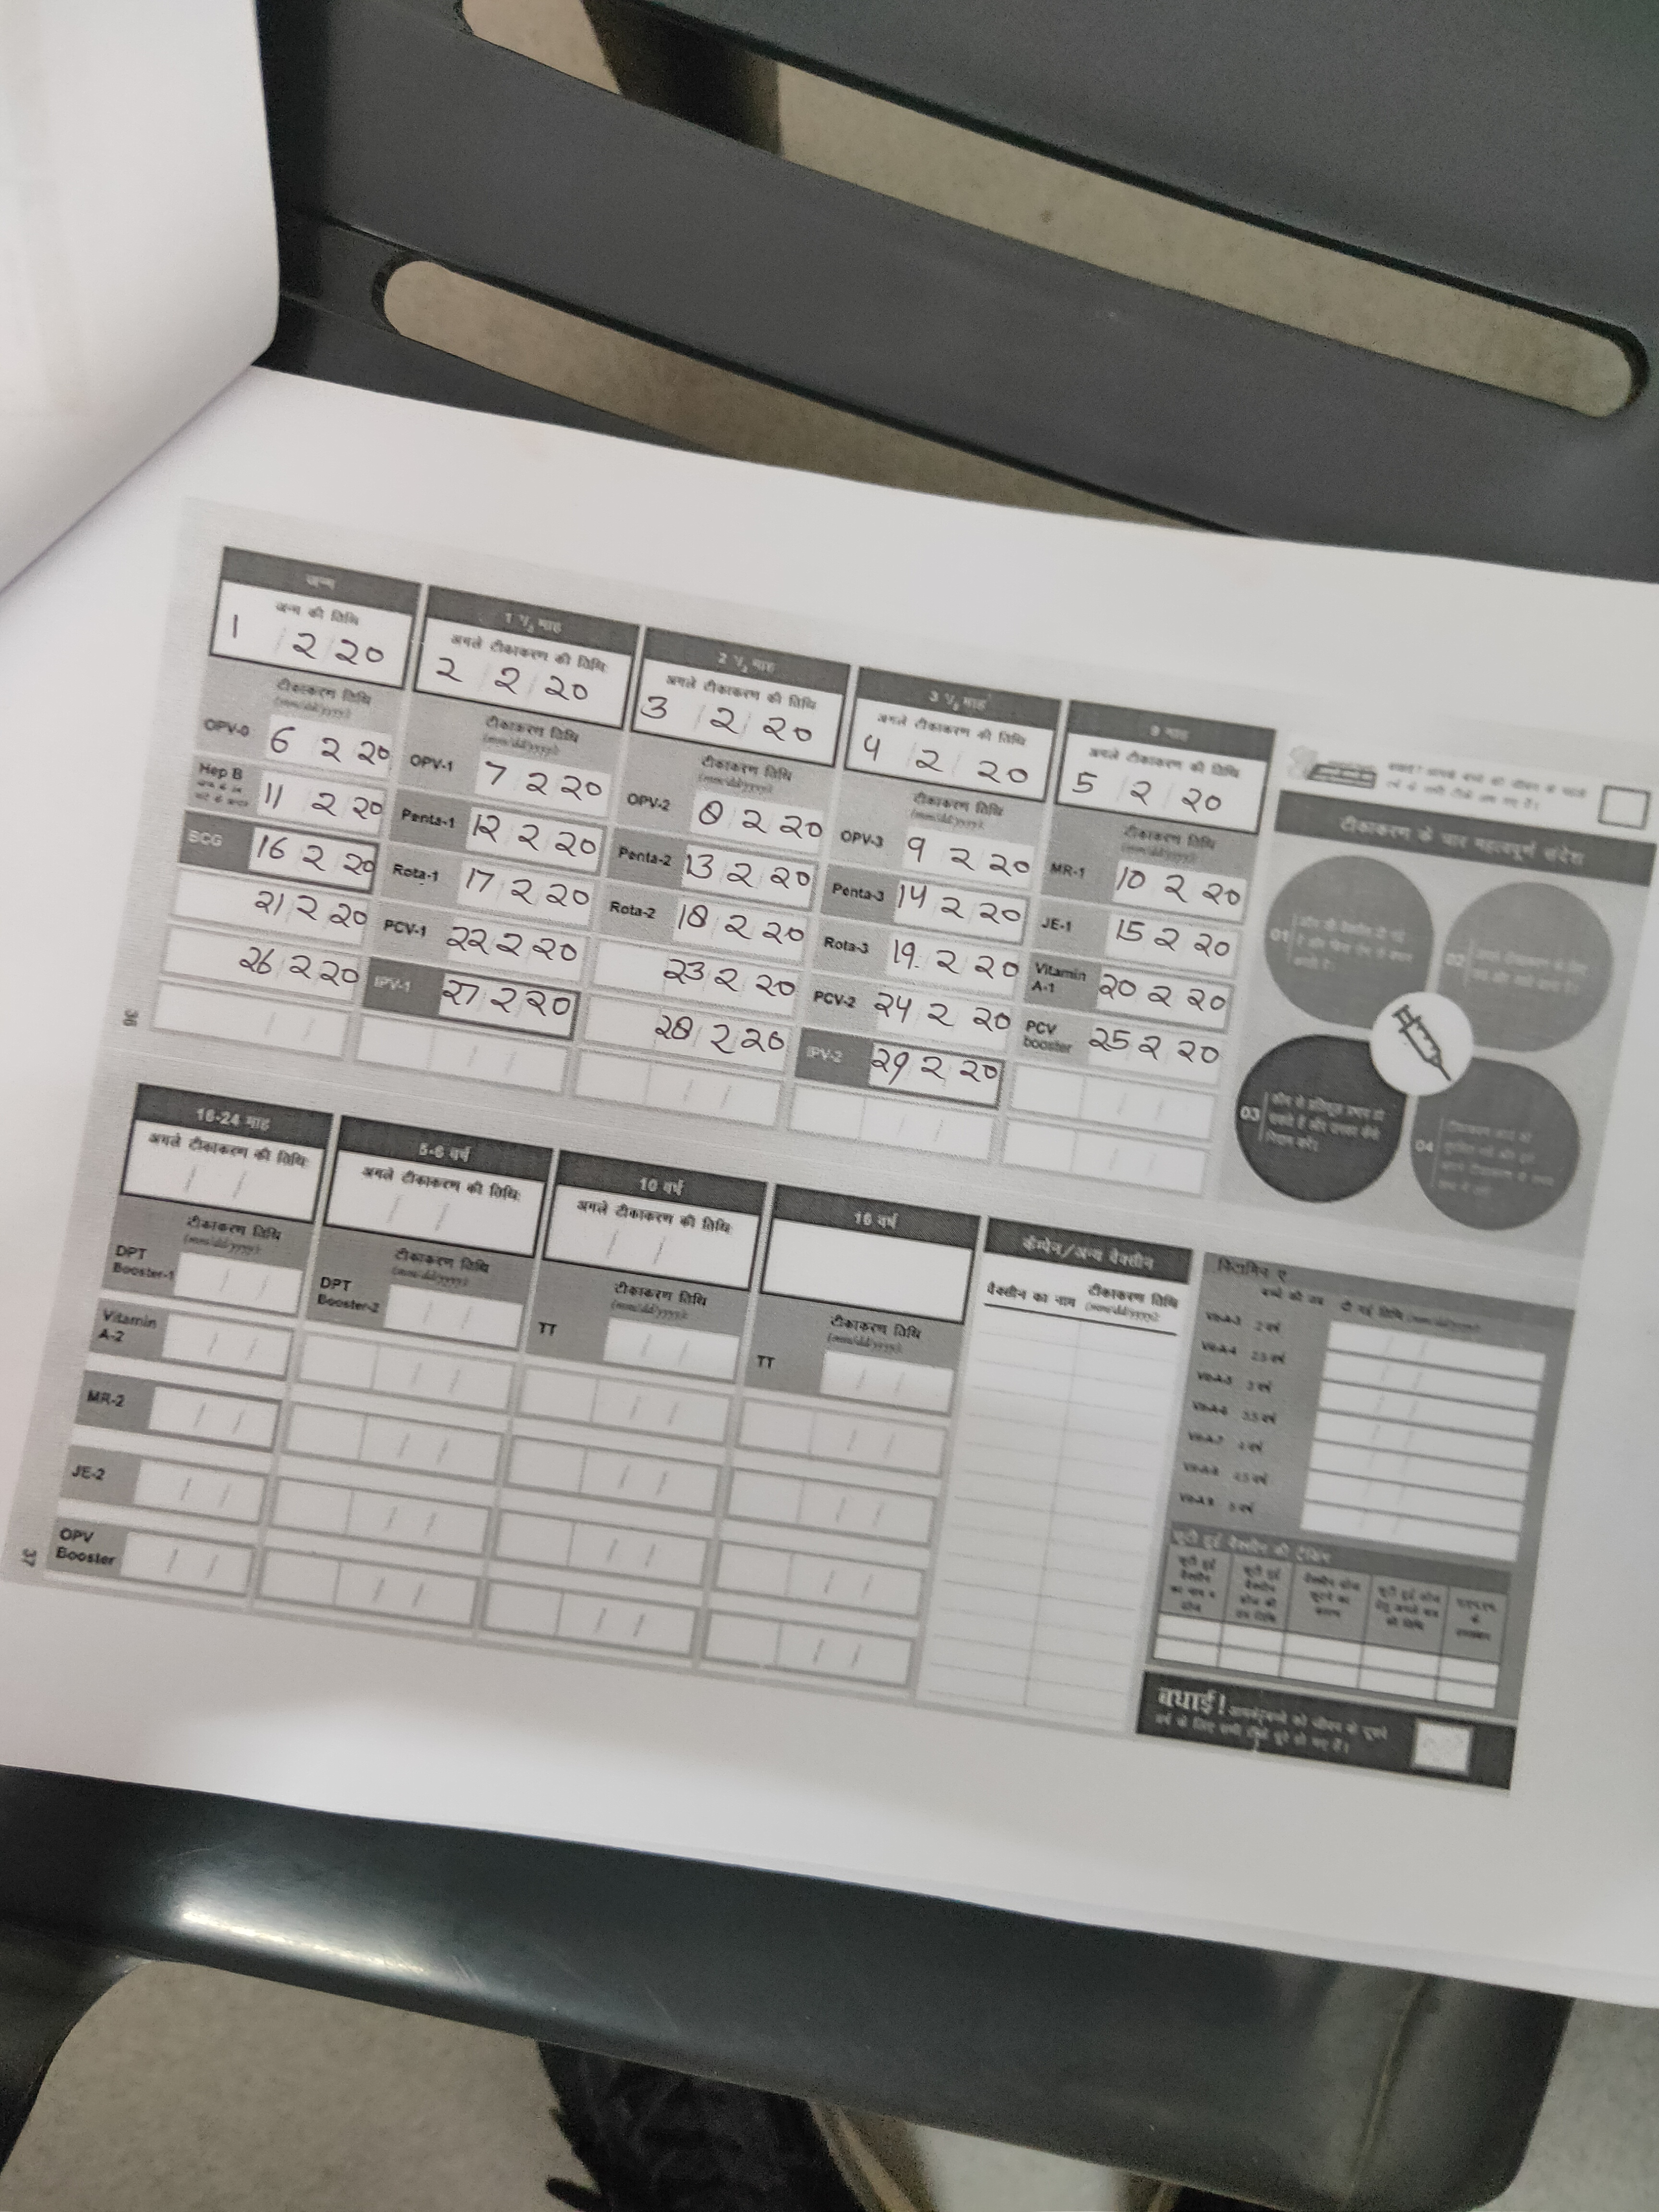
\includegraphics[scale=.065]{4/.report/_orig/p2.jpg}
      \caption{Printouts_2}
    \end{center}
    \endminipage
    \end{figure}
    \begin{figure}[!htb]
    %
    \minipage{\textwidth}
    \begin{center}
      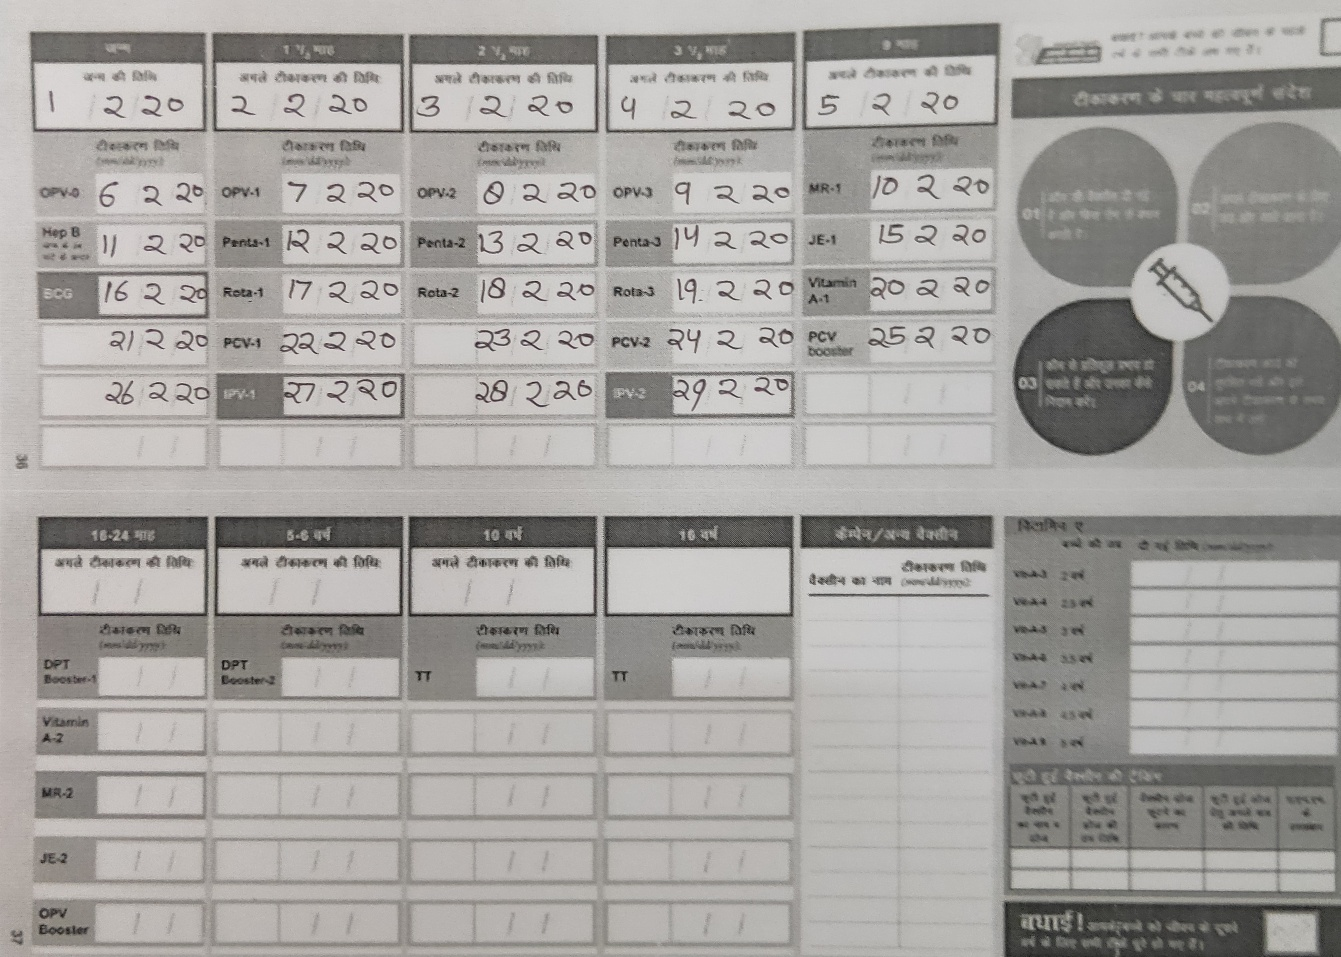
\includegraphics[scale=.2]{4/.report/_aligned/p2.jpg}
      \caption{Aligned}
    \end{center}
    \endminipage
    \end{figure}

% -------------------------------------------------------
\pagebreak
    \begin{figure}[!htb]
    %
    \minipage{\textwidth}
    \begin{center}
      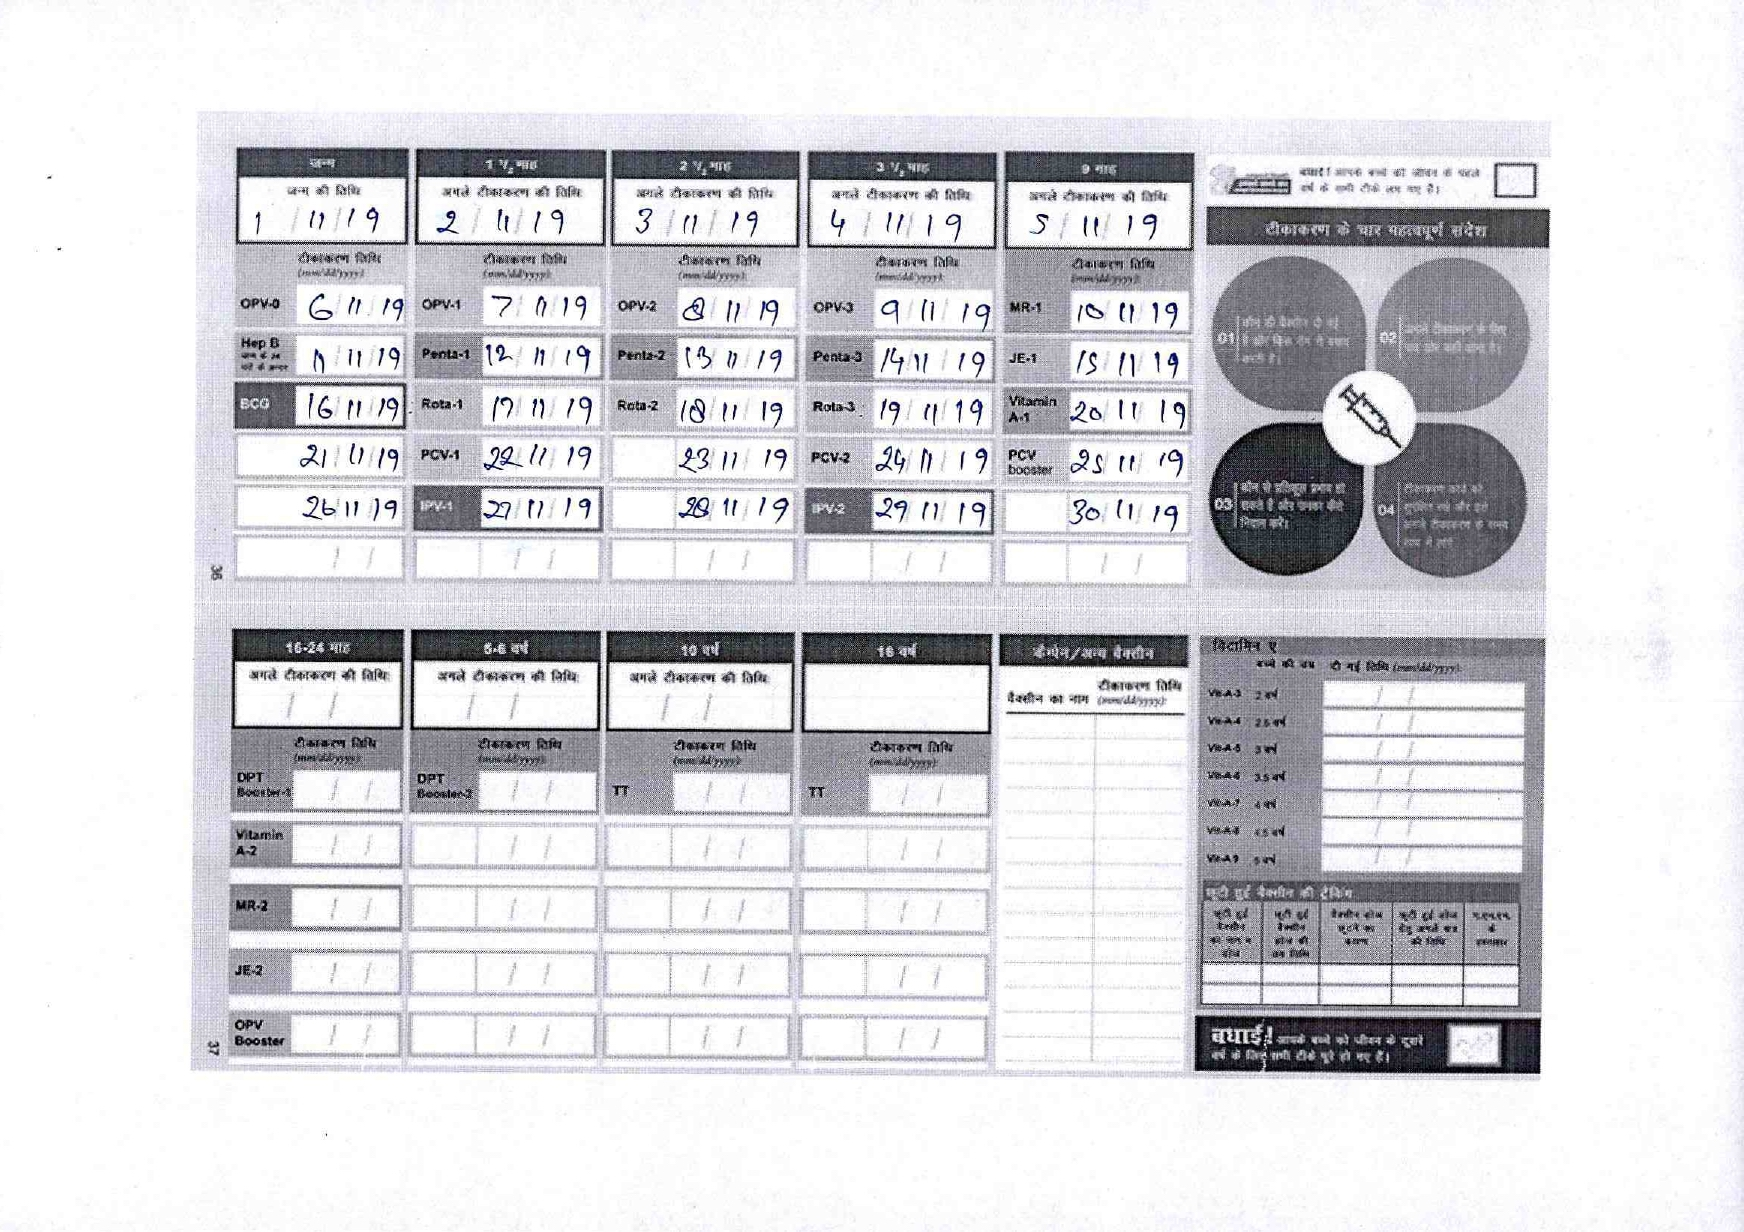
\includegraphics[scale=.25]{4/.report/_orig/s1.jpg}
      \caption{Scanned1}
    \end{center}
    \endminipage
    \end{figure}
    \begin{figure}[!htb]
    %
    \minipage{\textwidth}
    \begin{center}
      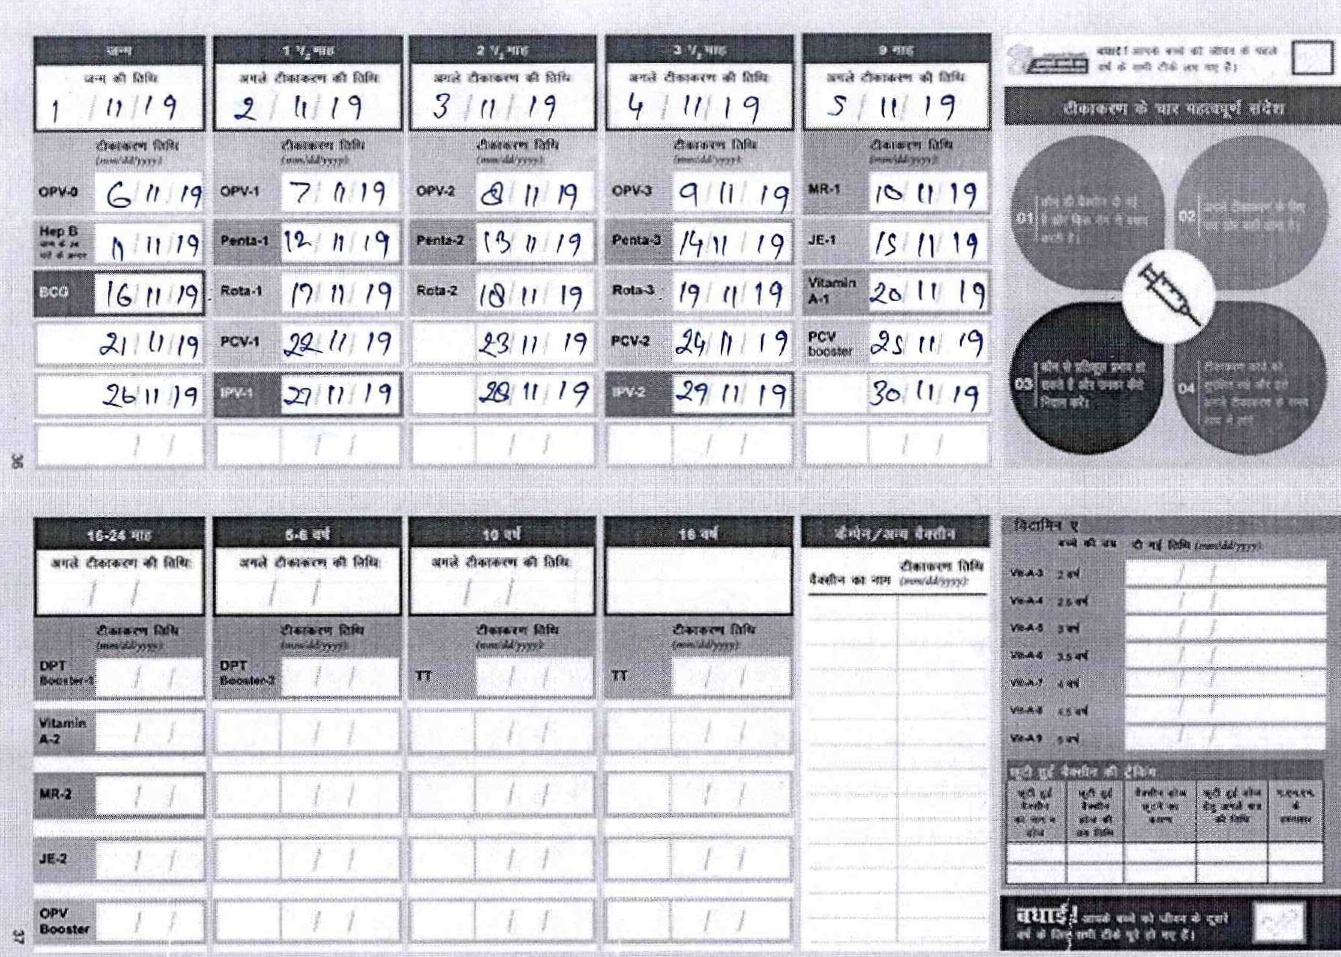
\includegraphics[scale=.2]{4/.report/_aligned/s1.jpg}
      \caption{Aligned}
    \end{center}
    \endminipage
    \end{figure}

% -------------------------------------------------------
\pagebreak
    \begin{figure}[!htb]
    %
    \minipage{\textwidth}
    \begin{center}
      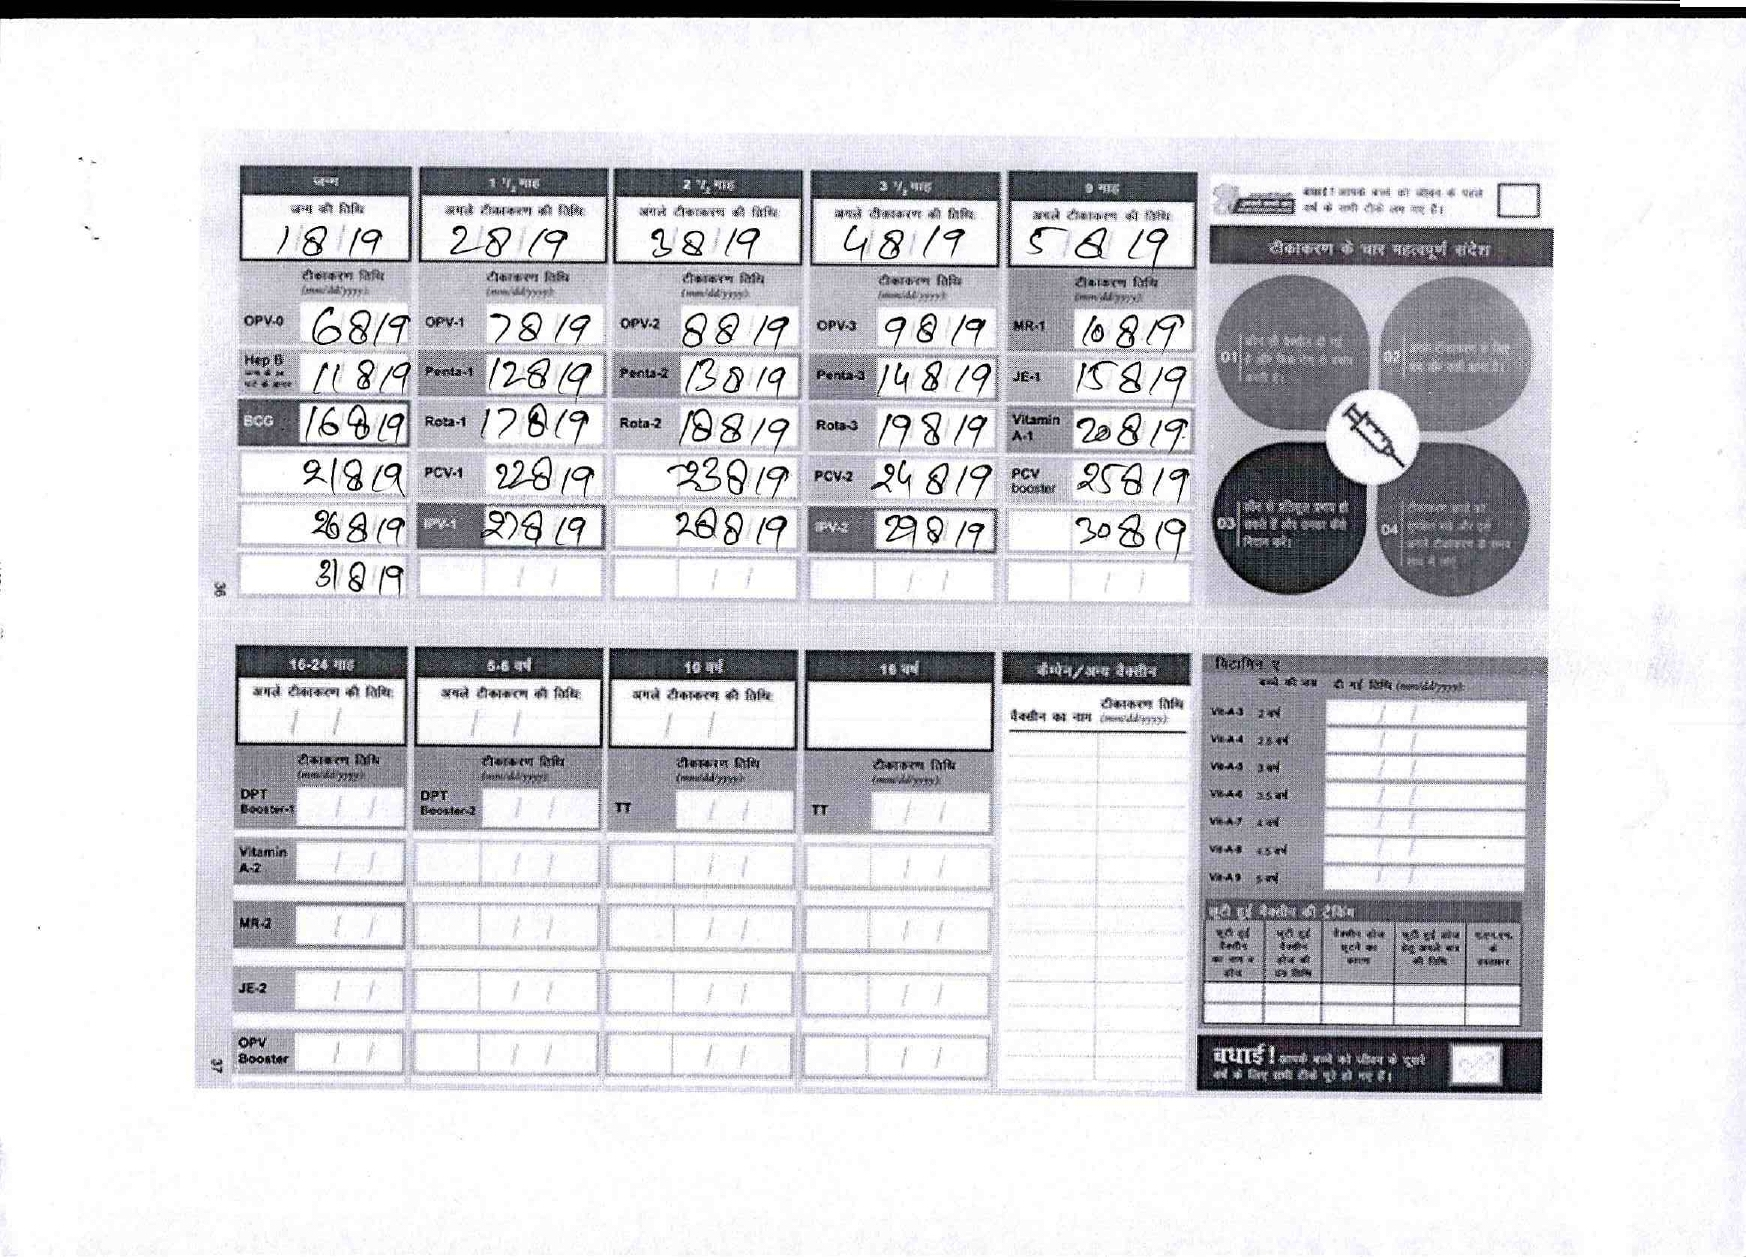
\includegraphics[scale=.25]{4/.report/_orig/s2.jpg}
      \caption{Scanned2}
    \end{center}
    \endminipage
    \end{figure}
    \begin{figure}[!htb]
    %
    \minipage{\textwidth}
    \begin{center}
      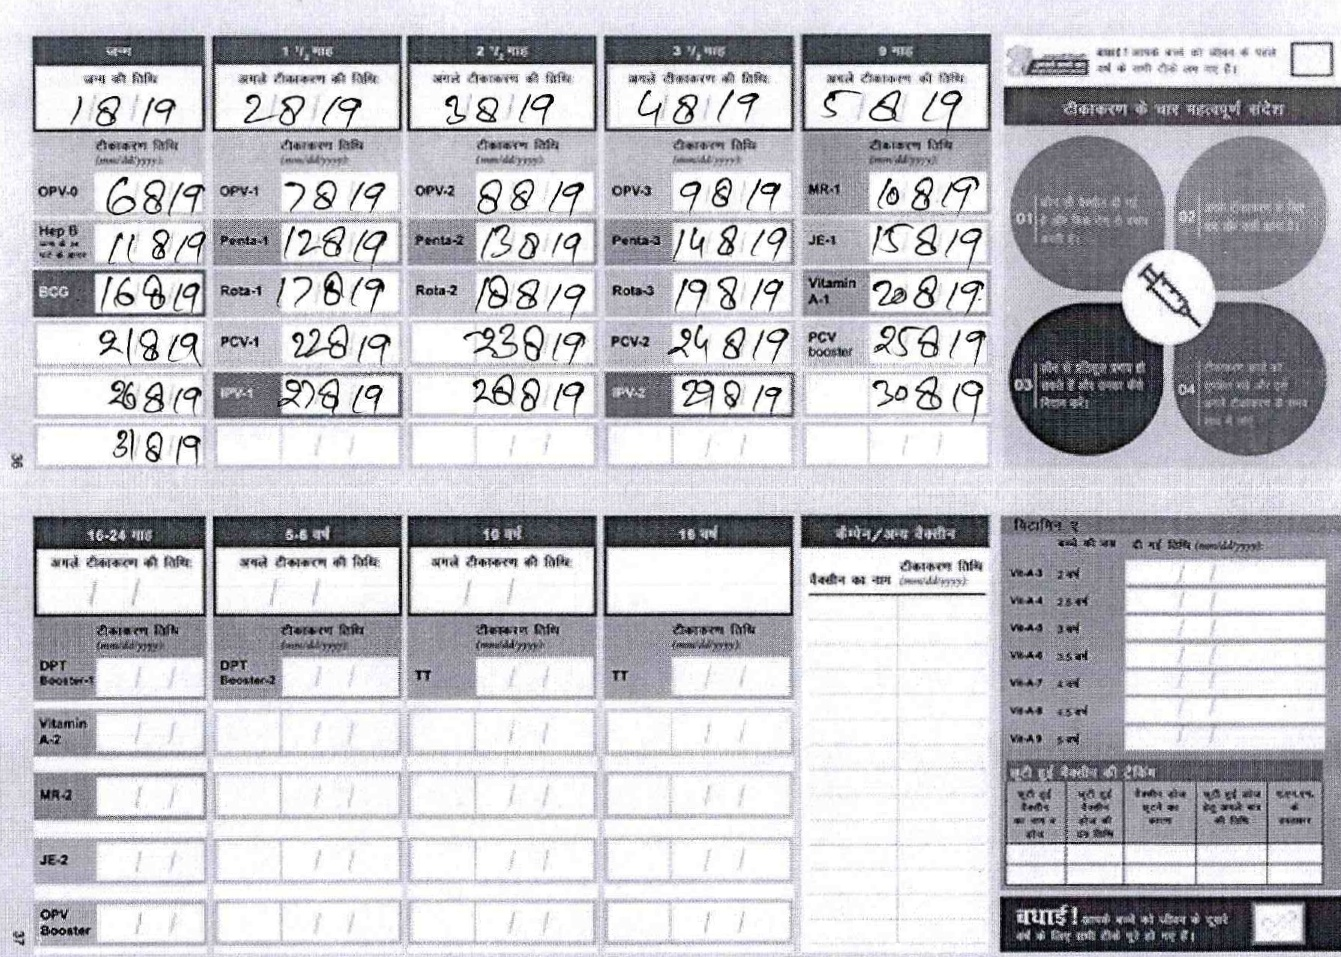
\includegraphics[scale=.2]{4/.report/_aligned/s2.jpg}
      \caption{Aligned}
    \end{center}
    \endminipage
    \end{figure}

% -------------------------------------------------------
\pagebreak
    \begin{figure}[!htb]
    %
    \minipage{\textwidth}
    \begin{center}
      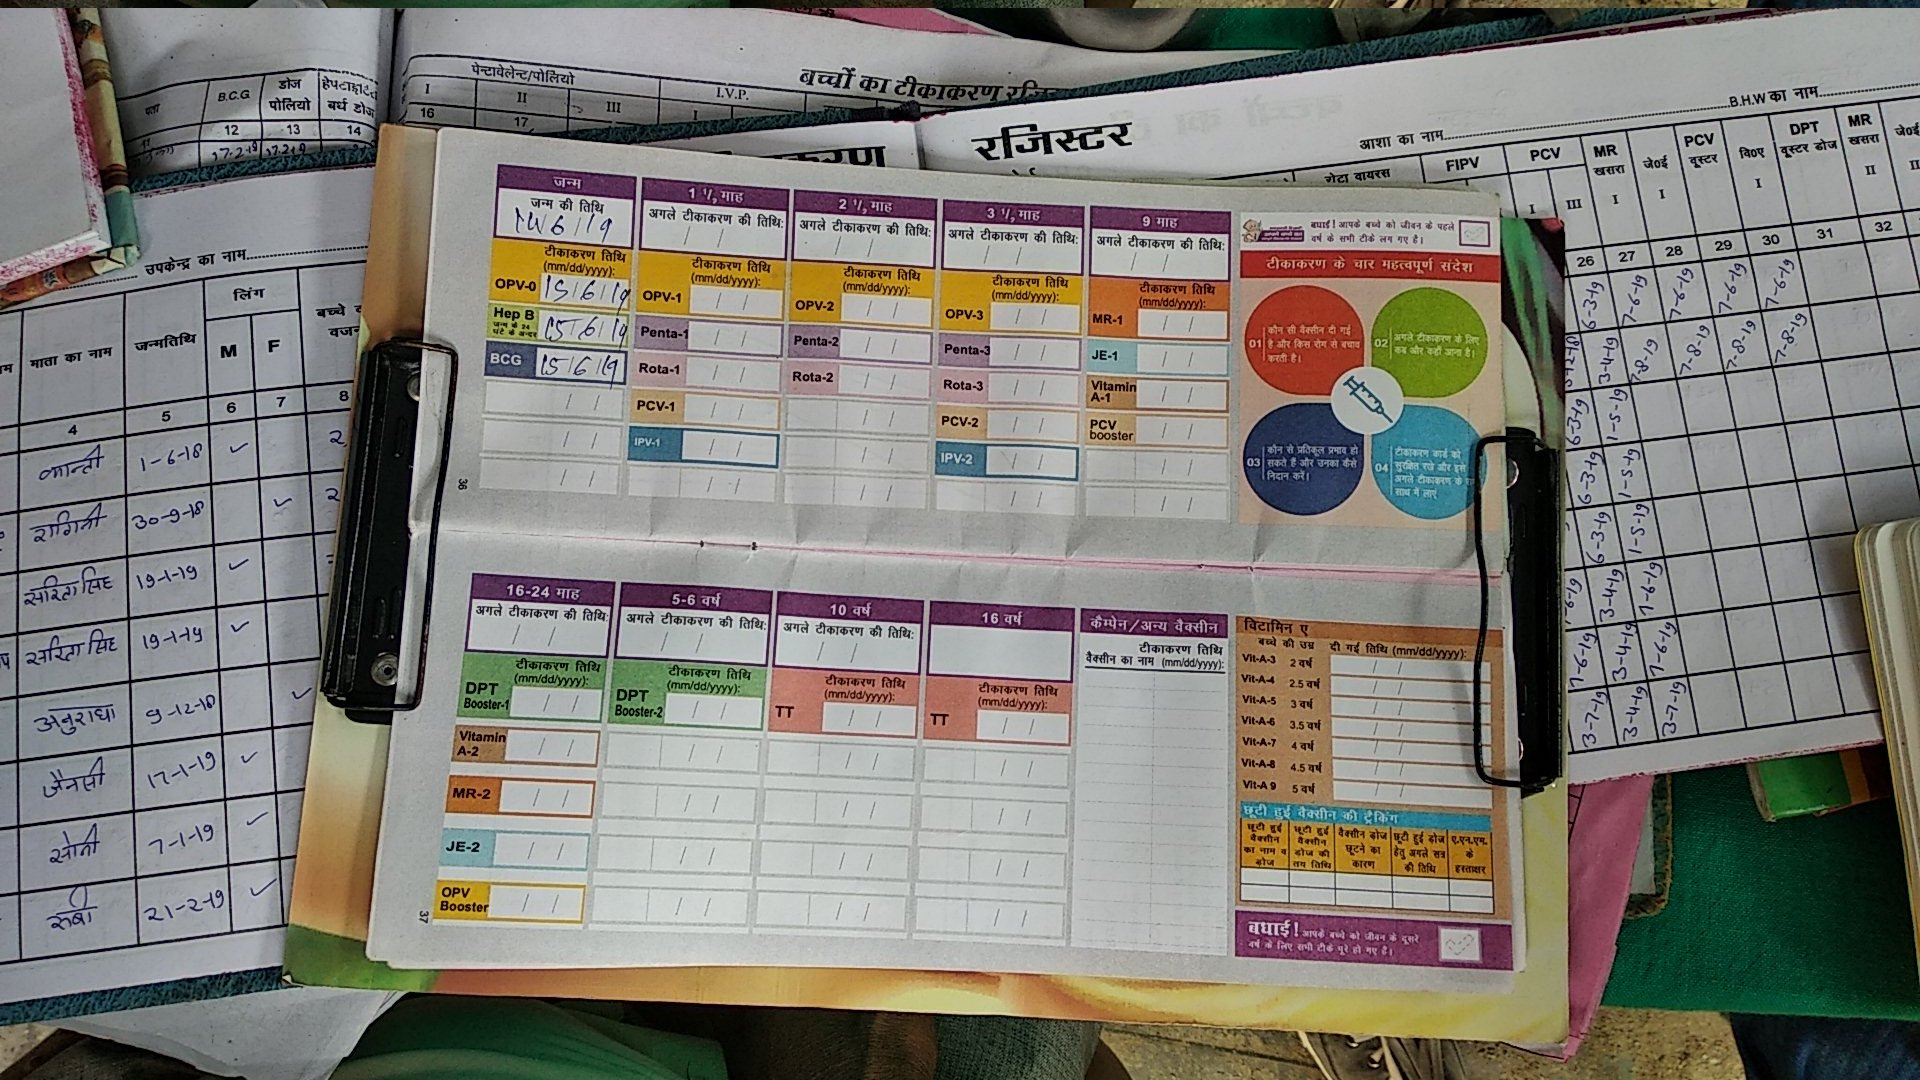
\includegraphics[scale=.25]{4/.report/_orig/b1.jpg}
      \caption{Booklet1}
    \end{center}
    \endminipage
    \end{figure}
    \begin{figure}[!htb]
    %
    \minipage{\textwidth}
    \begin{center}
      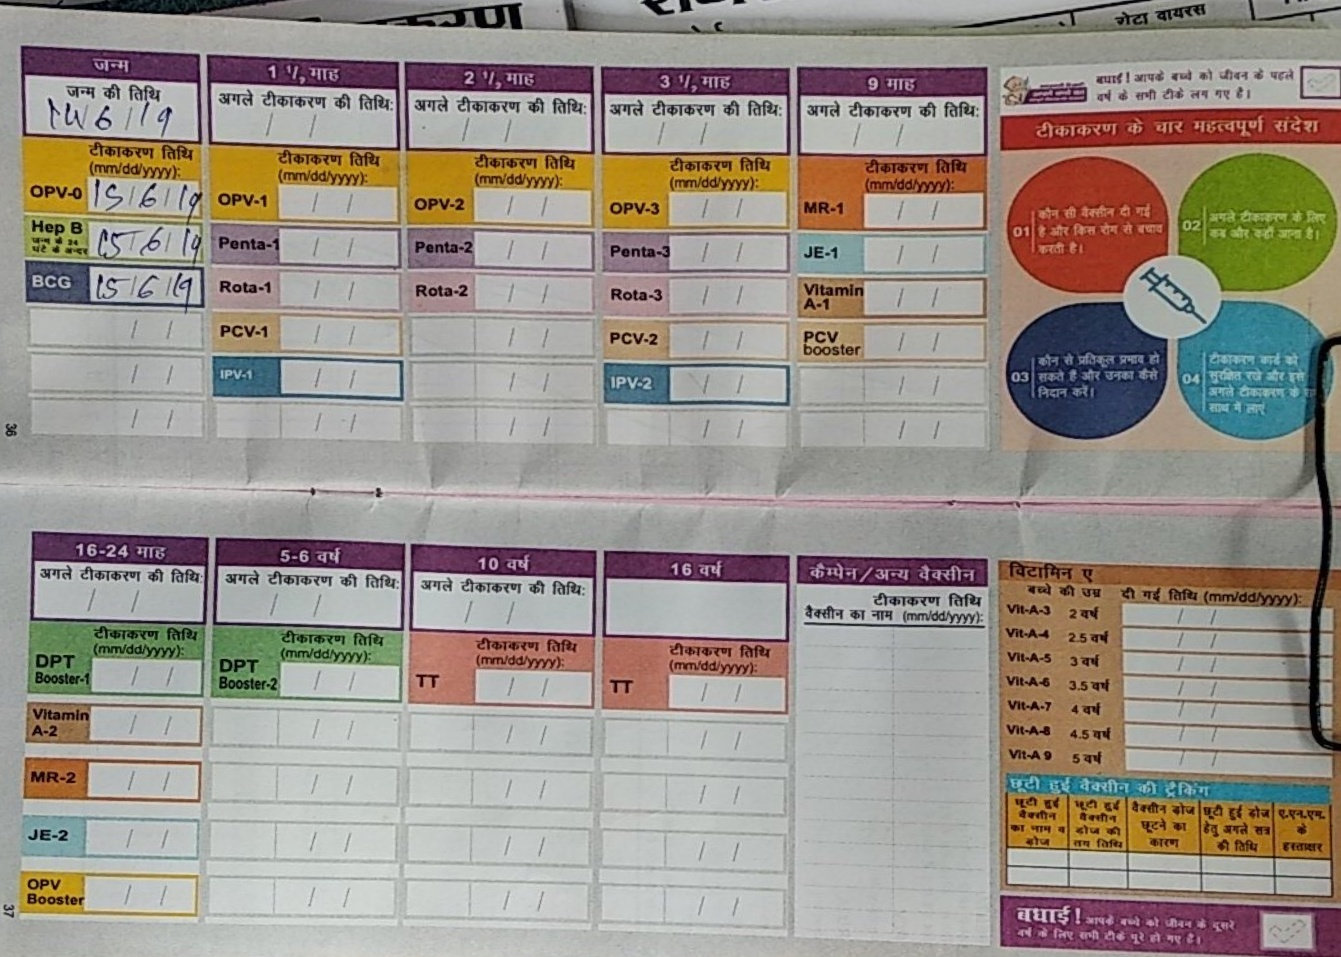
\includegraphics[scale=.2]{4/.report/_aligned/b1.jpg}
      \caption{Aligned}
    \end{center}
    \endminipage
    \end{figure}

% -------------------------------------------------------
\pagebreak
    \begin{figure}[!htb]
    %
    \minipage{\textwidth}
    \begin{center}
      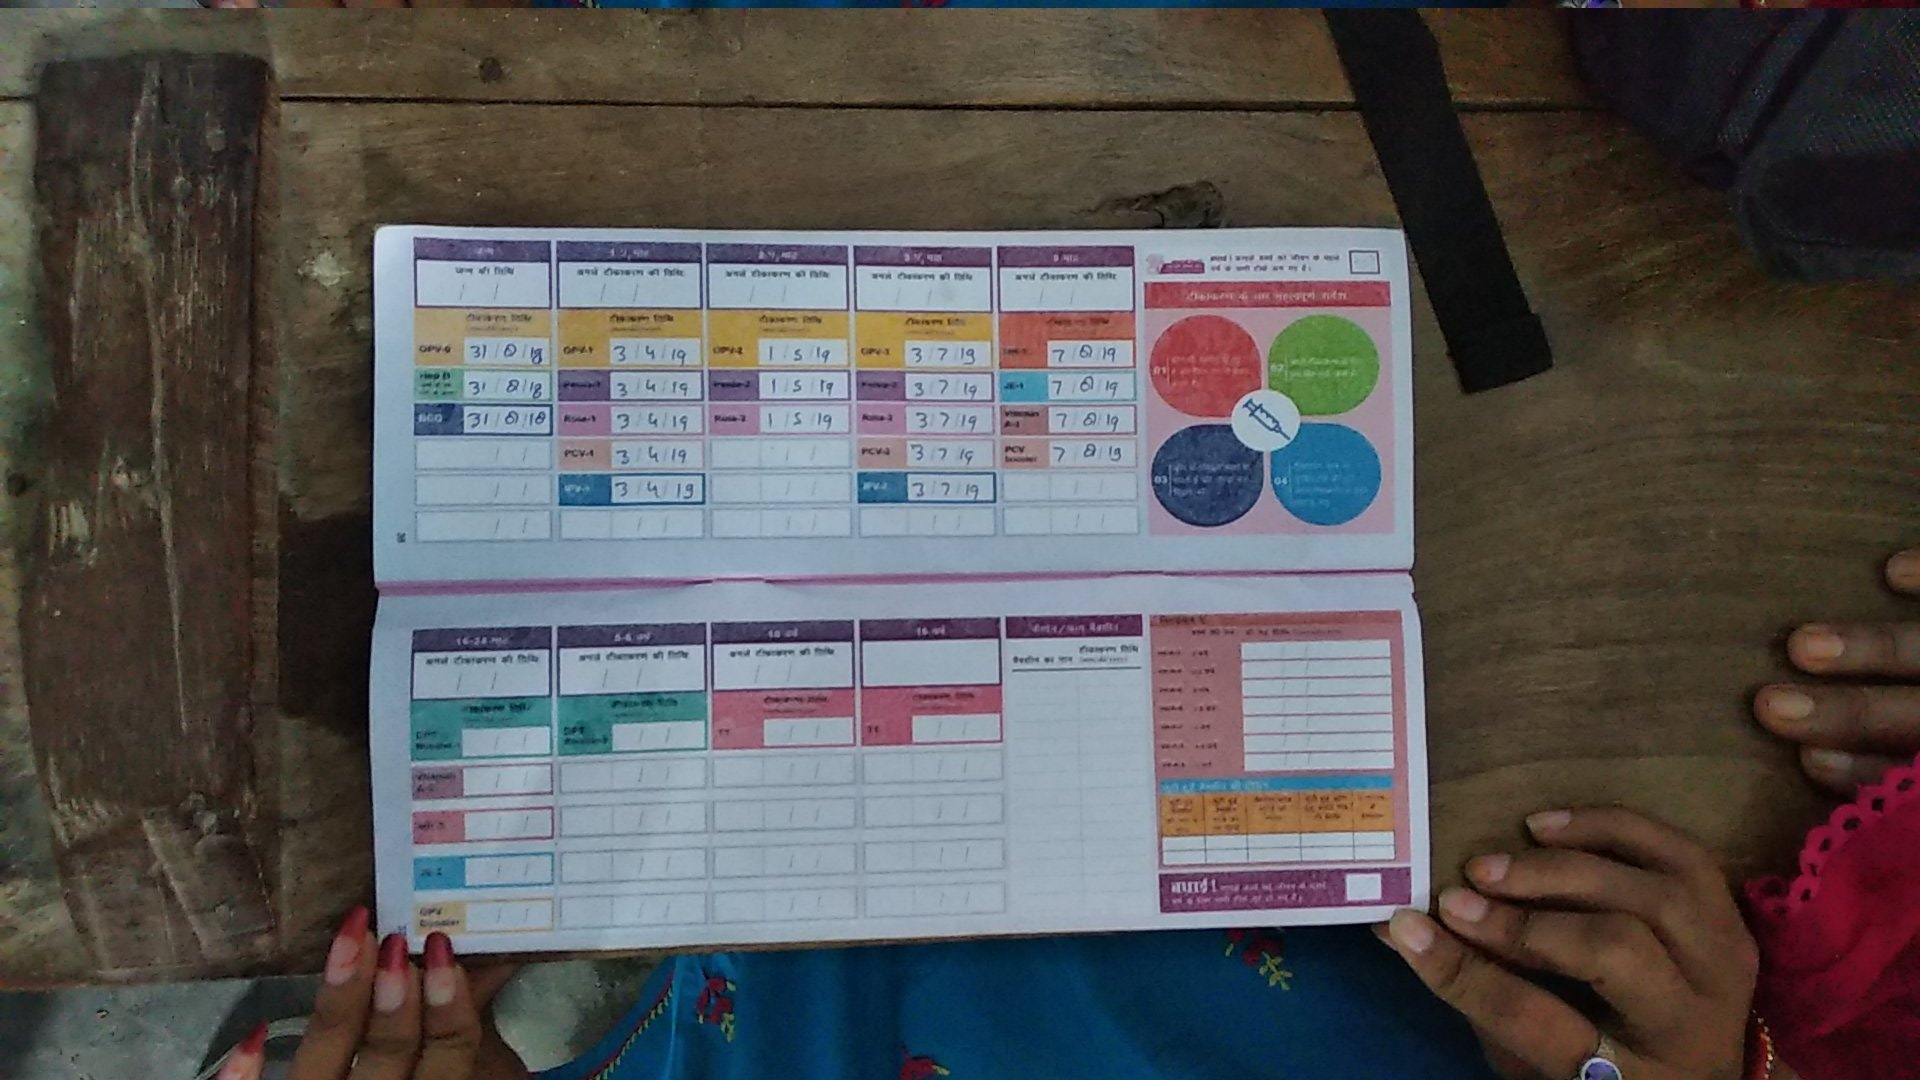
\includegraphics[scale=.25]{4/.report/_orig/b2.jpg}
      \caption{Booklet2}
    \end{center}
    \endminipage
    \end{figure}
    \begin{figure}[!htb]
    %
    \minipage{\textwidth}
    \begin{center}
      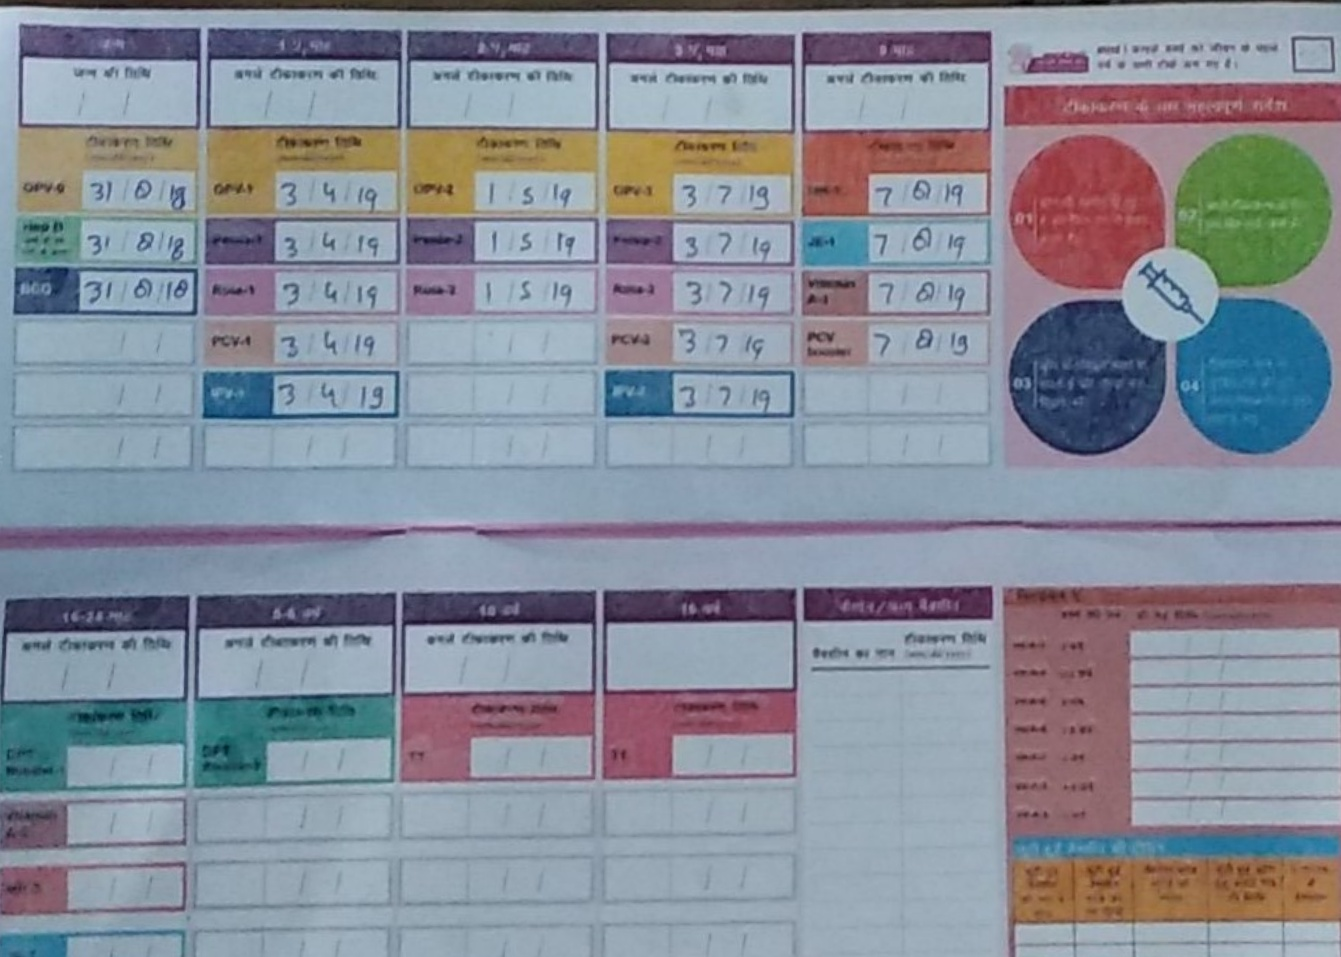
\includegraphics[scale=.2]{4/.report/_aligned/b2.jpg}
      \caption{Aligned}
    \end{center}
    \endminipage
    \end{figure}
% -------------------------------------------------------
% -------------------------------------------------------
% Topic I
    \pagebreak
    \subsection*{Image Segmentation}
% -------------------------------------------------------
    I tried, various approaches for segmenting the text fields from the complete image. Of these various attempts, I obtained decent results via two approaches, described below.\\
    \textbf{Contour Map}\\
    I implemented \texttt{Canny-Edge Detection} on the aligned image, and carved out boxes of desired aspect-ratio to get the boxes. This approach did work, but wasn't complete, i.e. many boxes were left out.\\
    \textbf{Predefined-Map}\\
    Since, the image alignment procedure, tries to warp most of the boxes in the same position, majority of boxes have fixed coordinates. I, thus, worked on a single image and through various measures (contouring) came up with the ideal mask for that image, but that mask can now be applied to all the images. This made segmentation very fast as well as majorly complete! The mask is presented below.\\
    Also, the results for both the procedures are presented below.
% -------------------------------------------------------
    
    \begin{figure}[!htb]
    \minipage{\textwidth}
    \begin{center}
        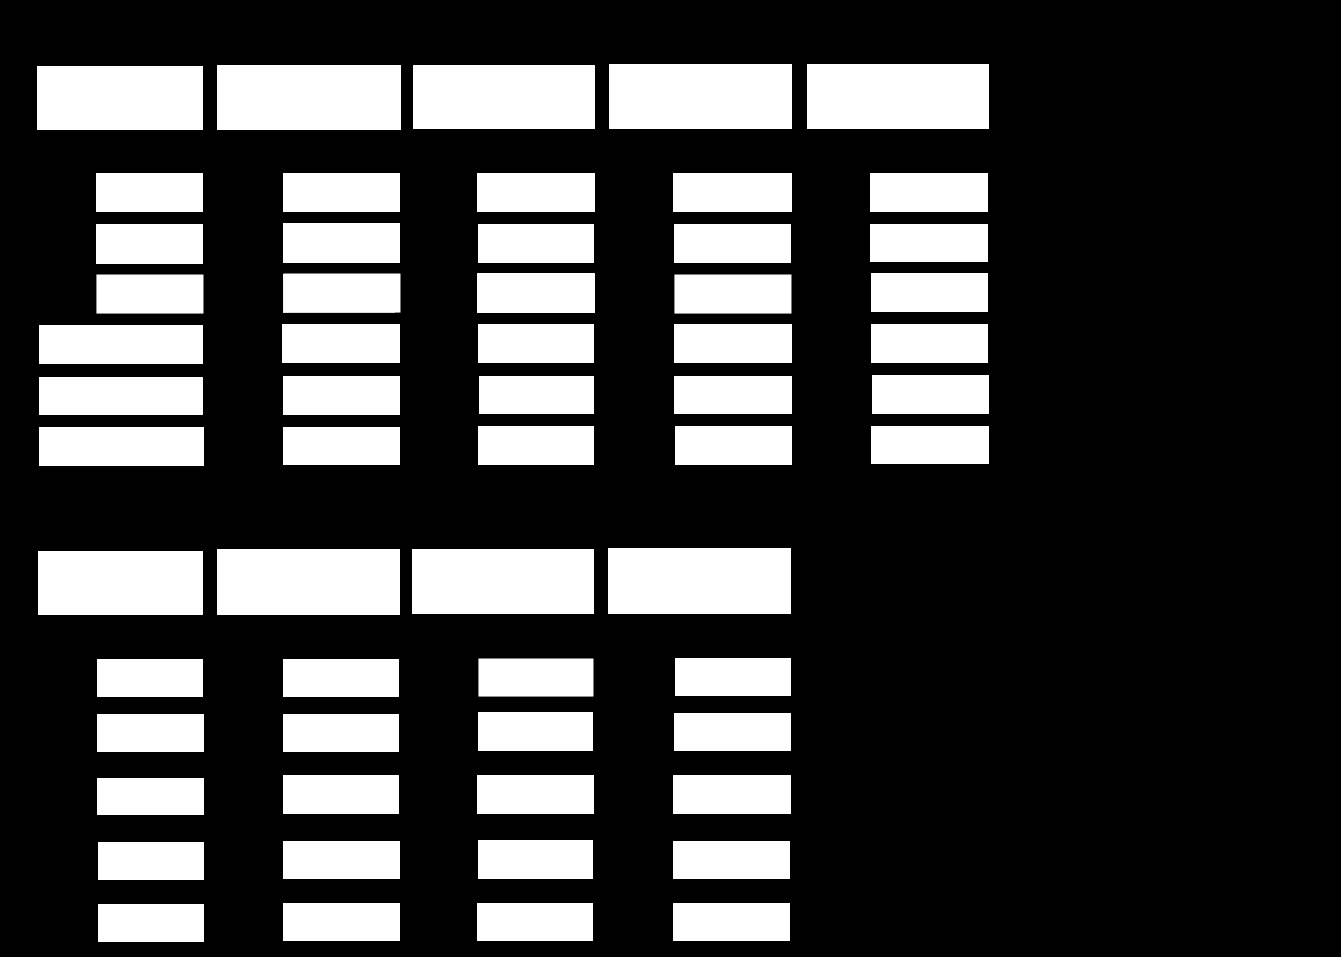
\includegraphics[scale=.25]{4/lib/best.png}
      \caption{Mask}
    \end{center}
    \endminipage \hfill
    \end{figure}
% -------------------------------------------------------
\pagebreak\\
\textbf{Contour Map}
    \begin{figure}[!htb]
    %
    \minipage{\textwidth}
    \begin{center}
      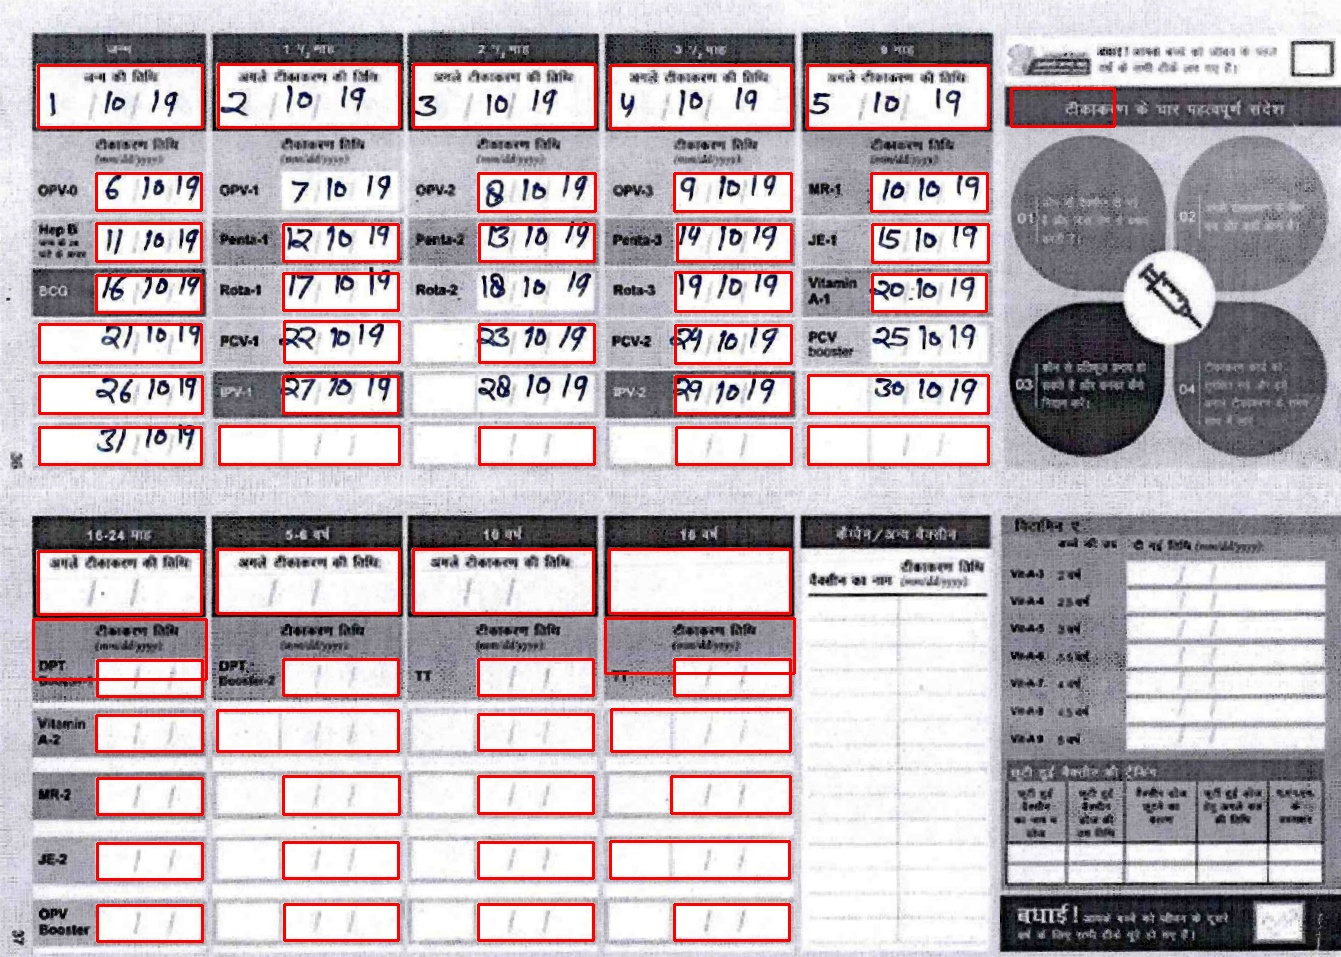
\includegraphics[scale=.25]{4/.report/_segmented/_cont/s1.jpg}
      \caption{Scanned1}
    \end{center}
    \endminipage
    \end{figure}
    \begin{figure}[!htb]
    %
    \minipage{\textwidth}
    \begin{center}
      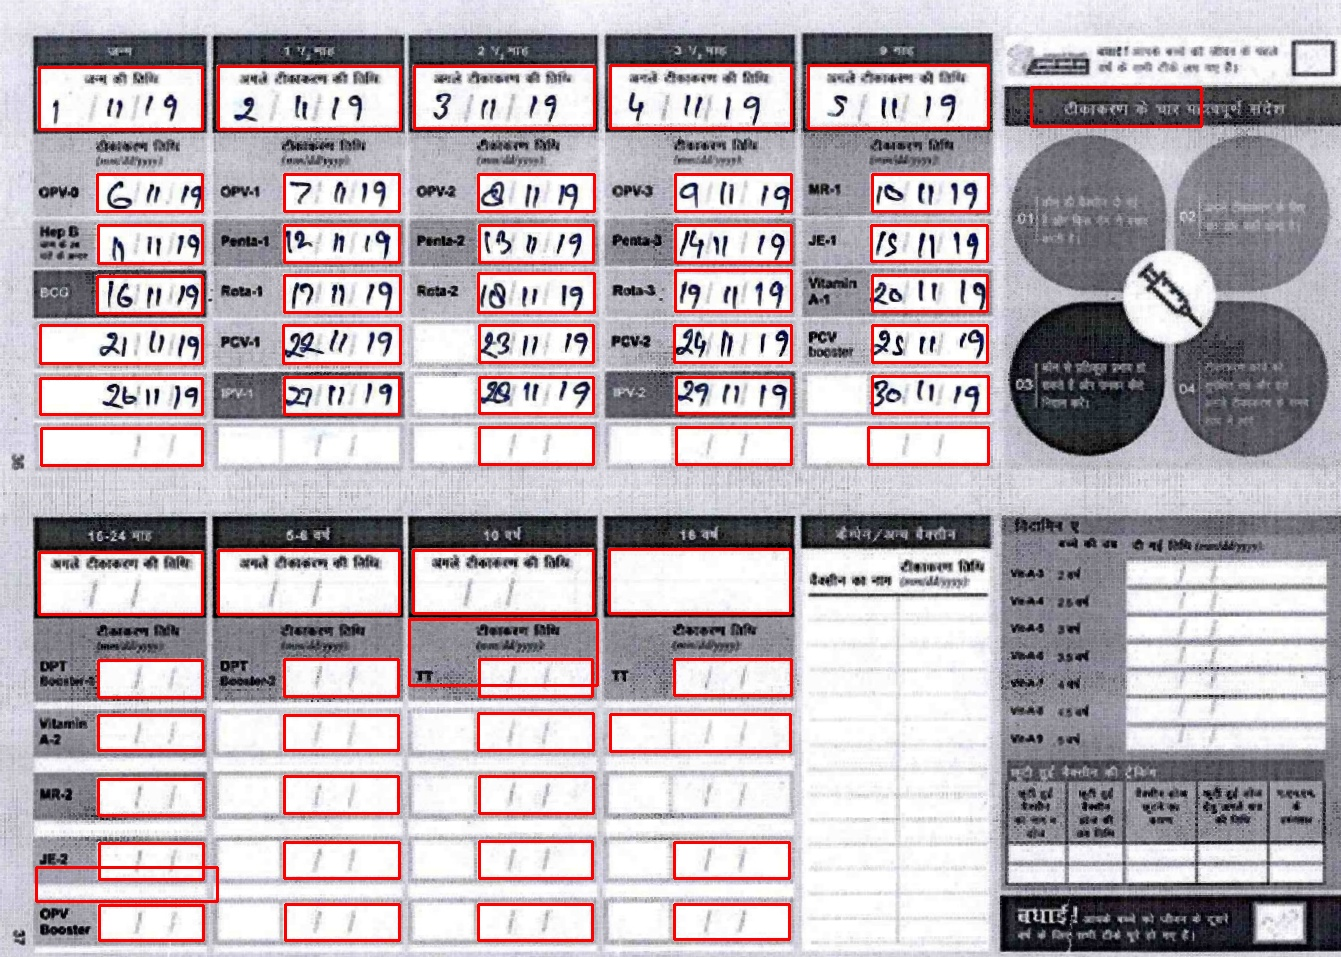
\includegraphics[scale=.25]{4/.report/_segmented/_cont/s2.jpg}
      \caption{Scanned2}
    \end{center}
    \endminipage
    \end{figure}
% -------------------------------------------------------
\pagebreak\\
\textbf{Contour Map}
    \begin{figure}[!htb]
    %
    \minipage{\textwidth}
    \begin{center}
      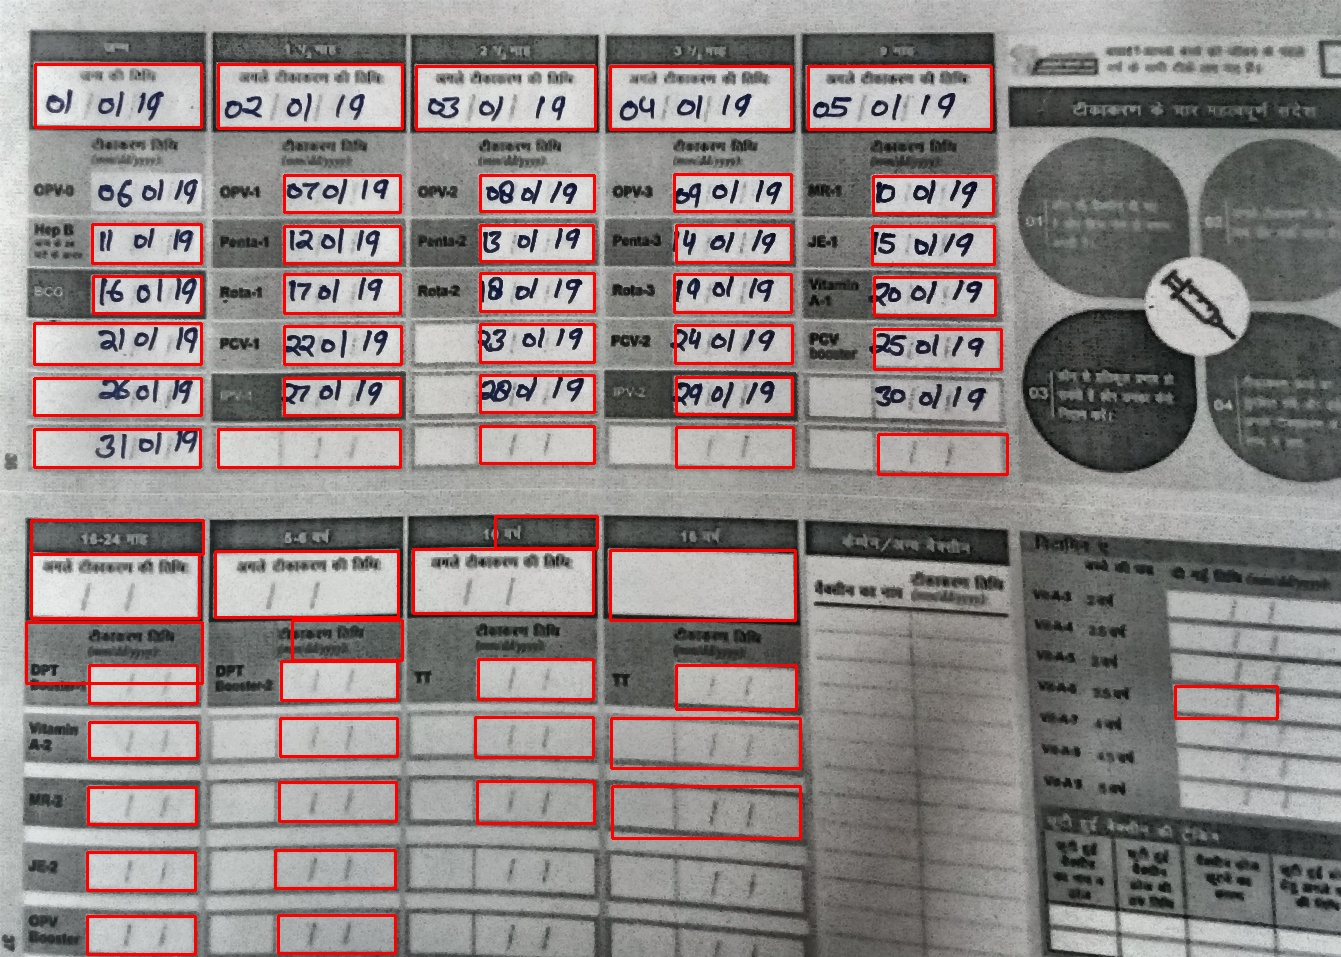
\includegraphics[scale=.25]{4/.report/_segmented/_cont/p1.jpg}
      \caption{Printout1}
    \end{center}
    \endminipage
    \end{figure}
    \begin{figure}[!htb]
    %
    \minipage{\textwidth}
    \begin{center}
      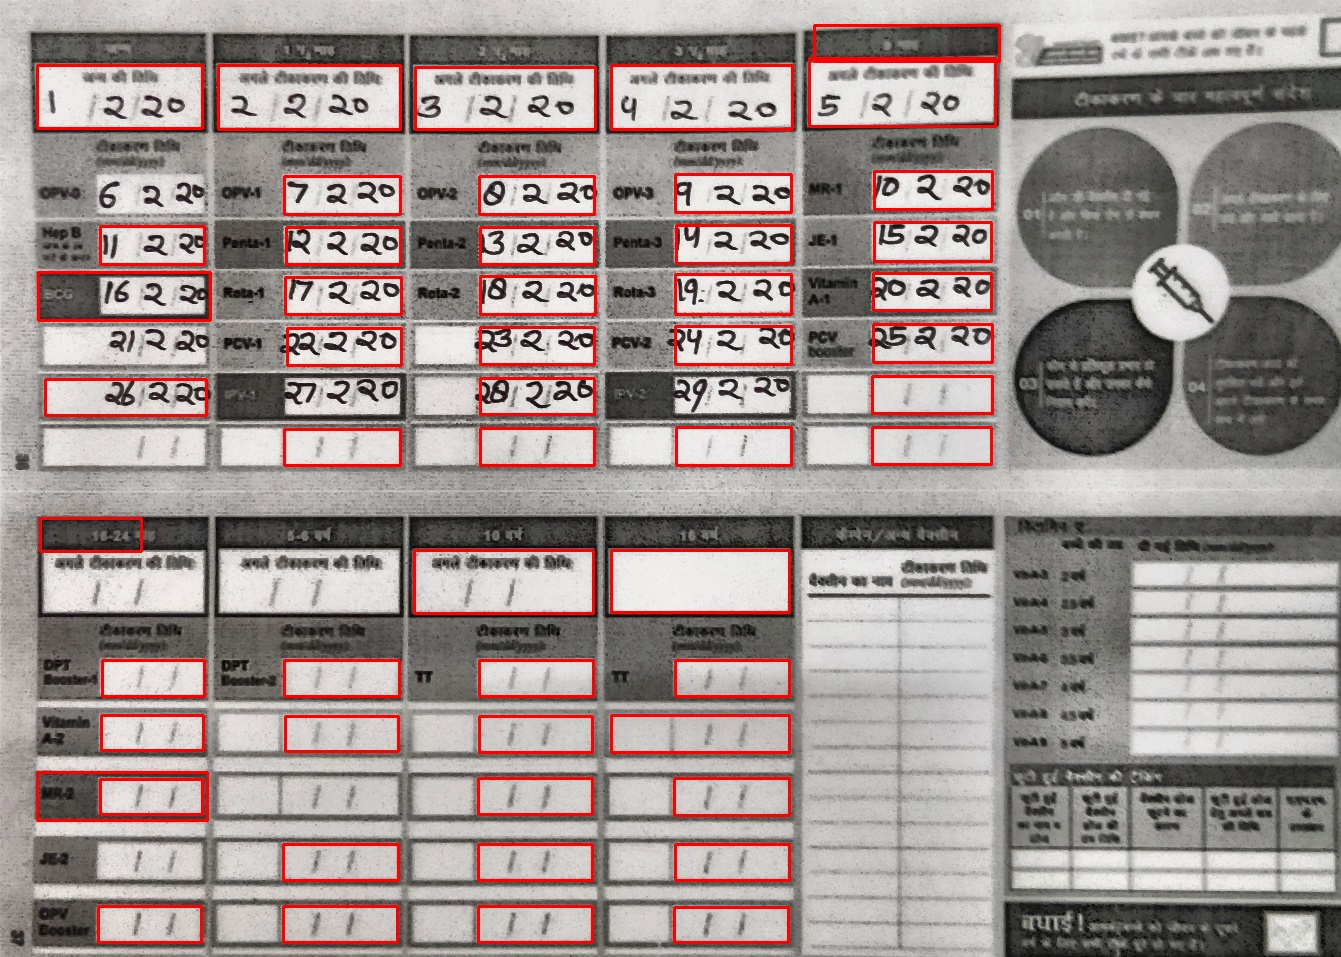
\includegraphics[scale=.25]{4/.report/_segmented/_cont/p2.jpg}
      \caption{Printout2}
    \end{center}
    \endminipage
    \end{figure}
% -------------------------------------------------------
\pagebreak \\
\textbf{Contour Map}
    \begin{figure}[!htb]
    %
    \minipage{\textwidth}
    \begin{center}
      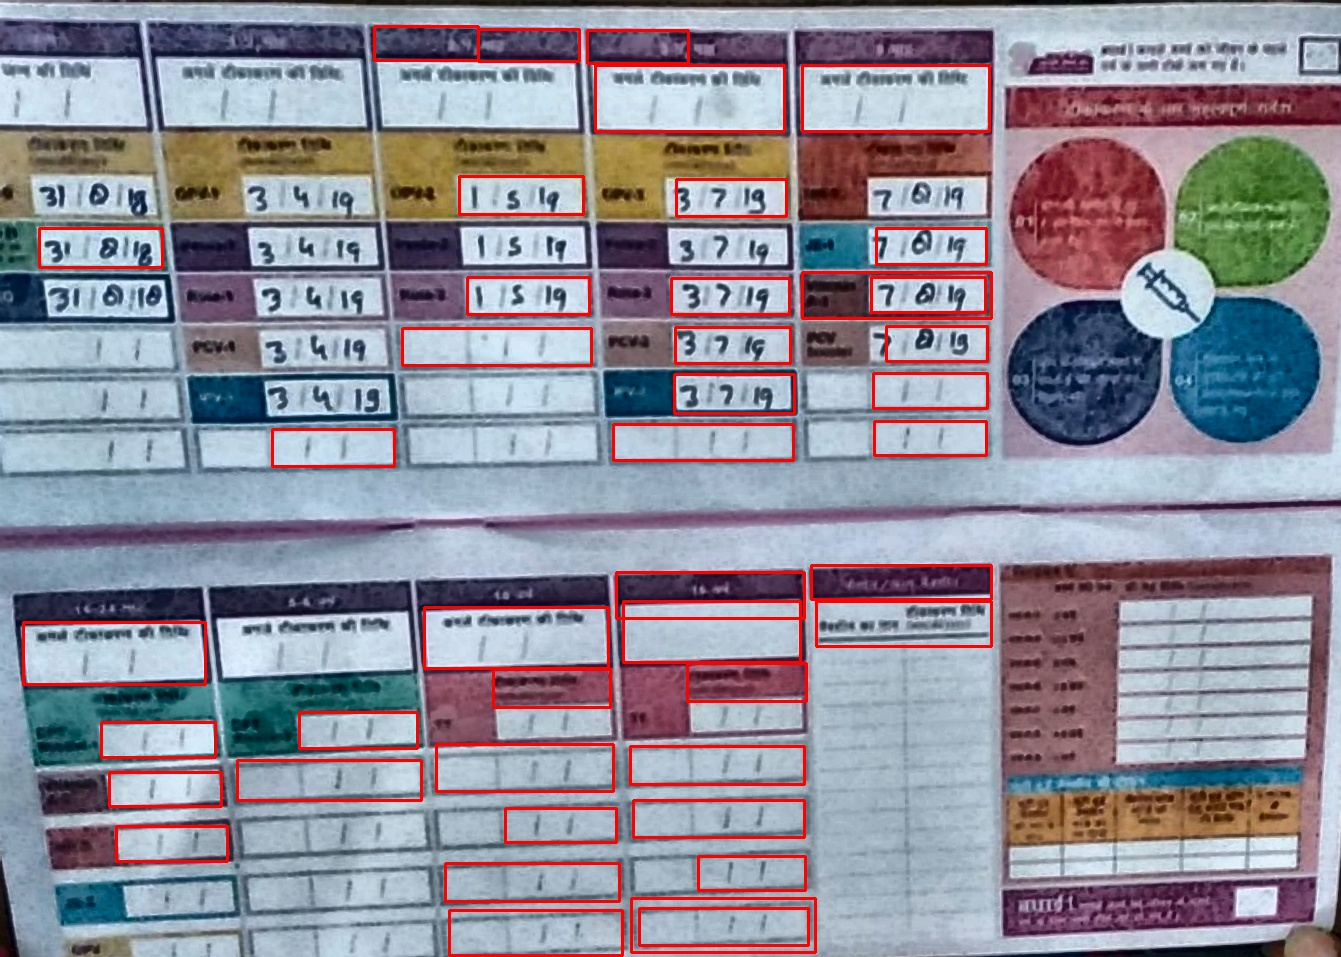
\includegraphics[scale=.25]{4/.report/_segmented/_cont/b1.jpg}
      \caption{Booklet1}
    \end{center}
    \endminipage
    \end{figure}
    \begin{figure}[!htb]
    %
    \minipage{\textwidth}
    \begin{center}
      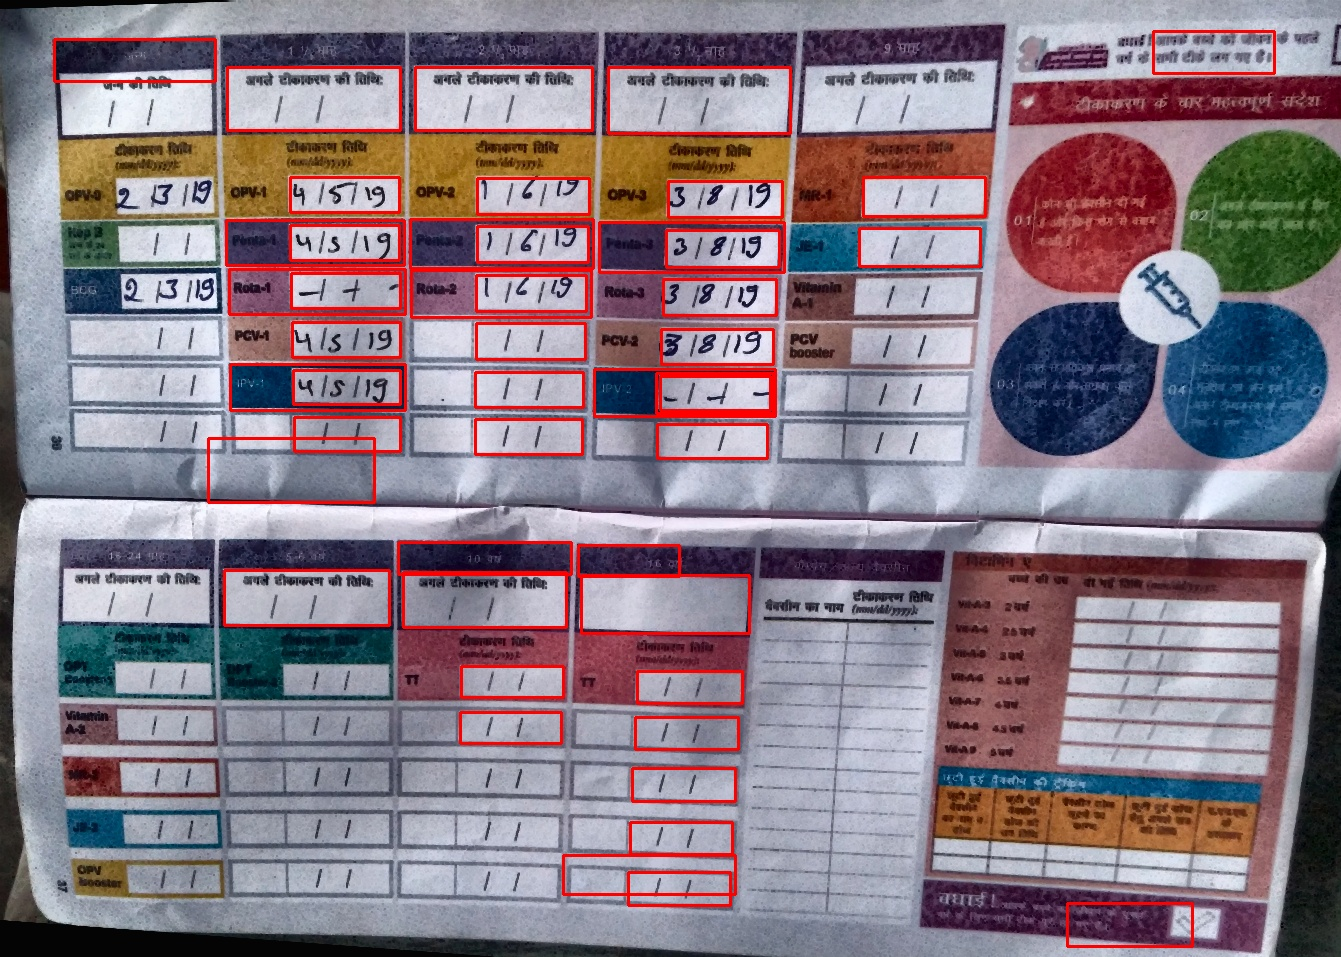
\includegraphics[scale=.25]{4/.report/_segmented/_cont/b2.jpg}
      \caption{Booklet2}
    \end{center}
    \endminipage
    \end{figure}
% ------------------------------------------------------- 
% -------------------------------------------------------
\pagebreak\\
\textbf{Masked}
    \begin{figure}[!htb]
    %
    \minipage{\textwidth}
    \begin{center}
      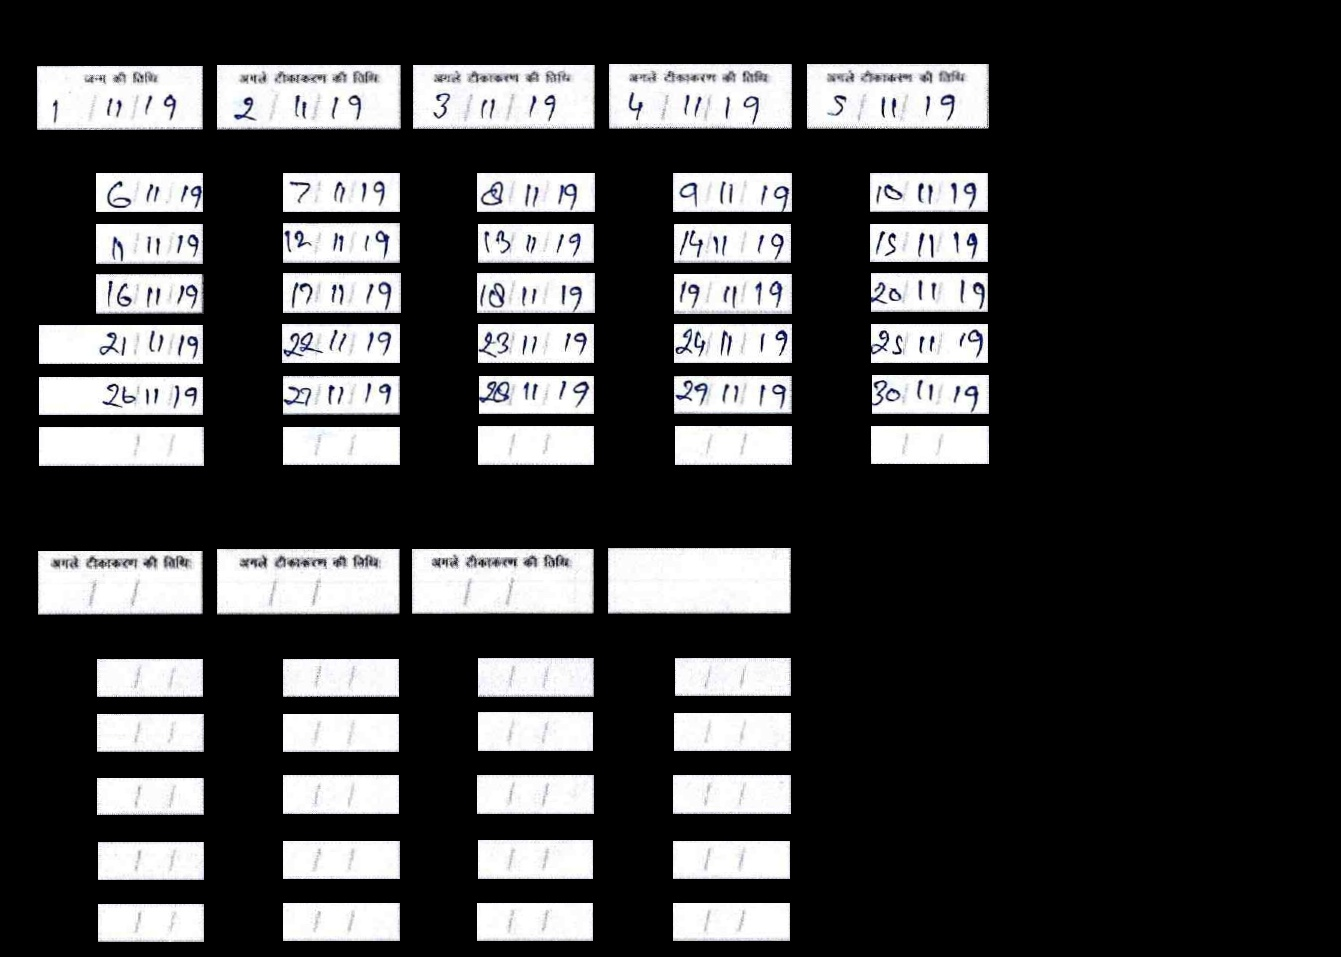
\includegraphics[scale=.25]{4/.report/_segmented/_mask/s1.jpg}
      \caption{Scanned1}
    \end{center}
    \endminipage
    \end{figure}
    \begin{figure}[!htb]
    %
    \minipage{\textwidth}
    \begin{center}
      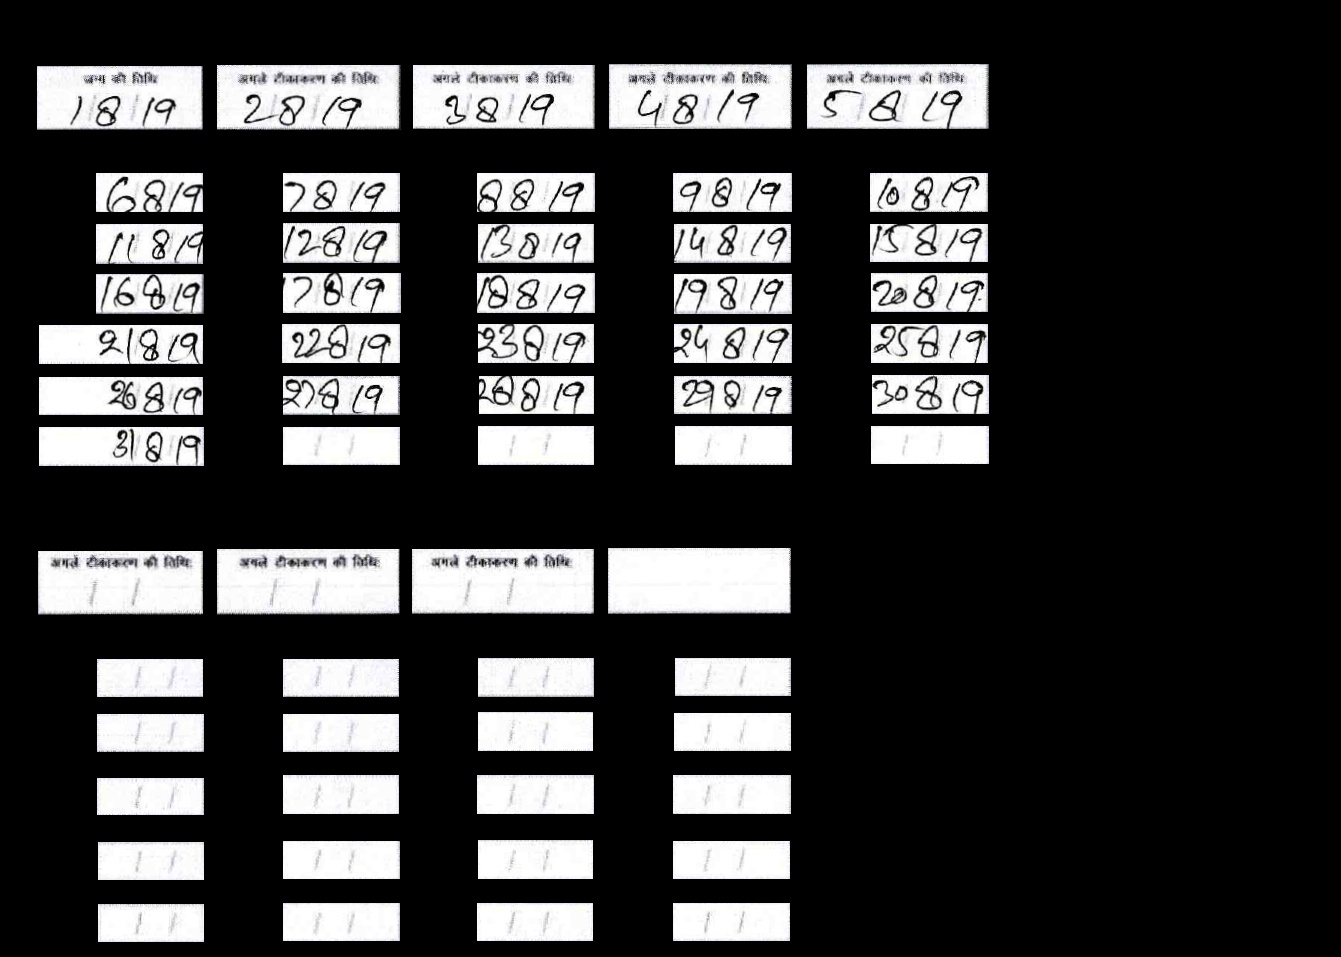
\includegraphics[scale=.25]{4/.report/_segmented/_mask/s2.jpg}
      \caption{Scanned2}
    \end{center}
    \endminipage
    \end{figure}
% -------------------------------------------------------
\pagebreak\\
\textbf{Masked}
    \begin{figure}[!htb]
    %
    \minipage{\textwidth}
    \begin{center}
      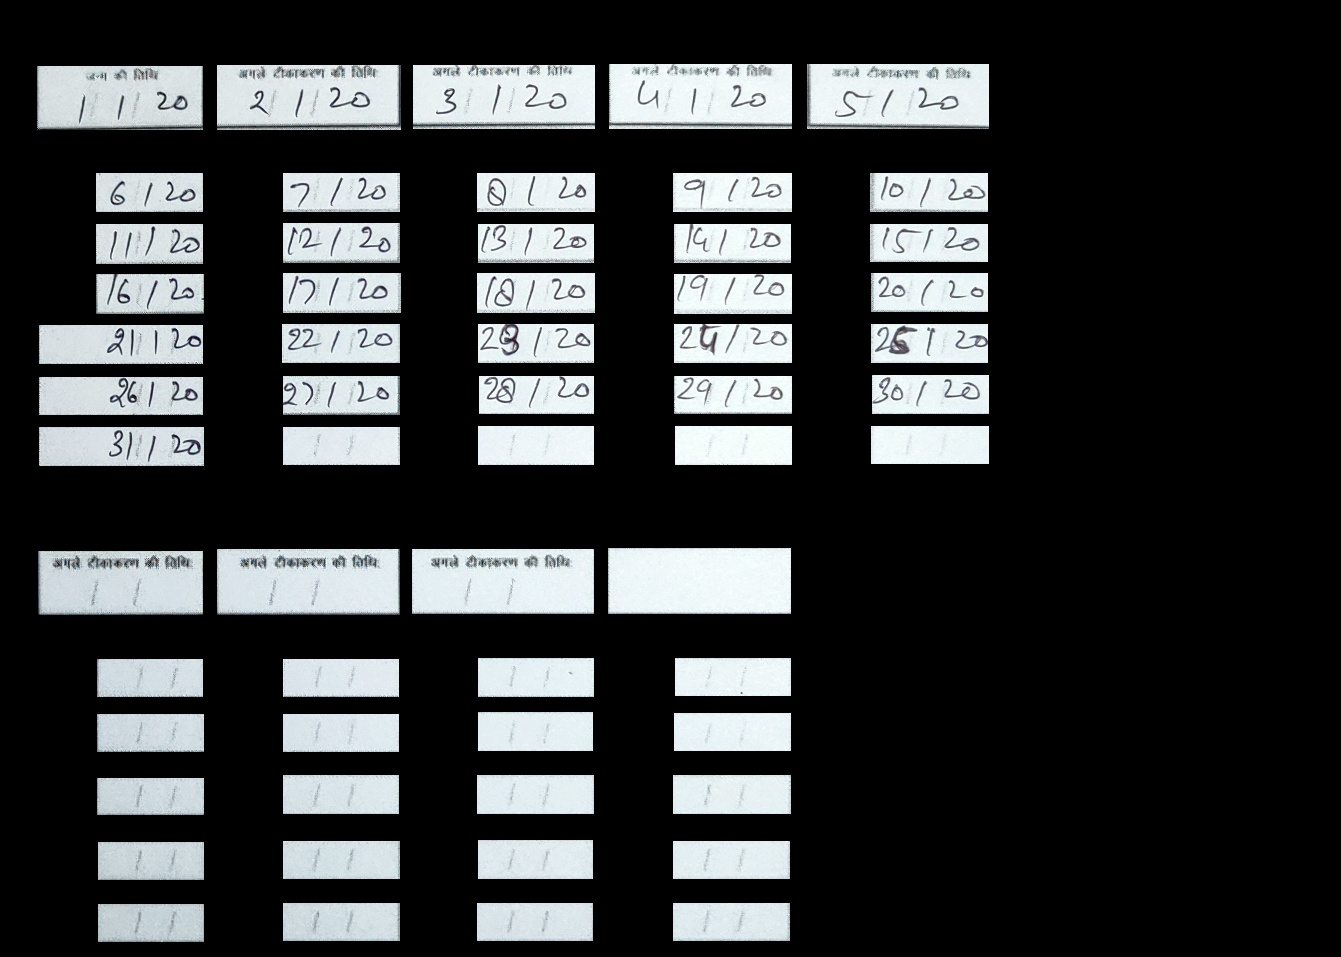
\includegraphics[scale=.25]{4/.report/_segmented/_mask/p1.jpg}
      \caption{Printout1}
    \end{center}
    \endminipage
    \end{figure}
    \begin{figure}[!htb]
    %
    \minipage{\textwidth}
    \begin{center}
      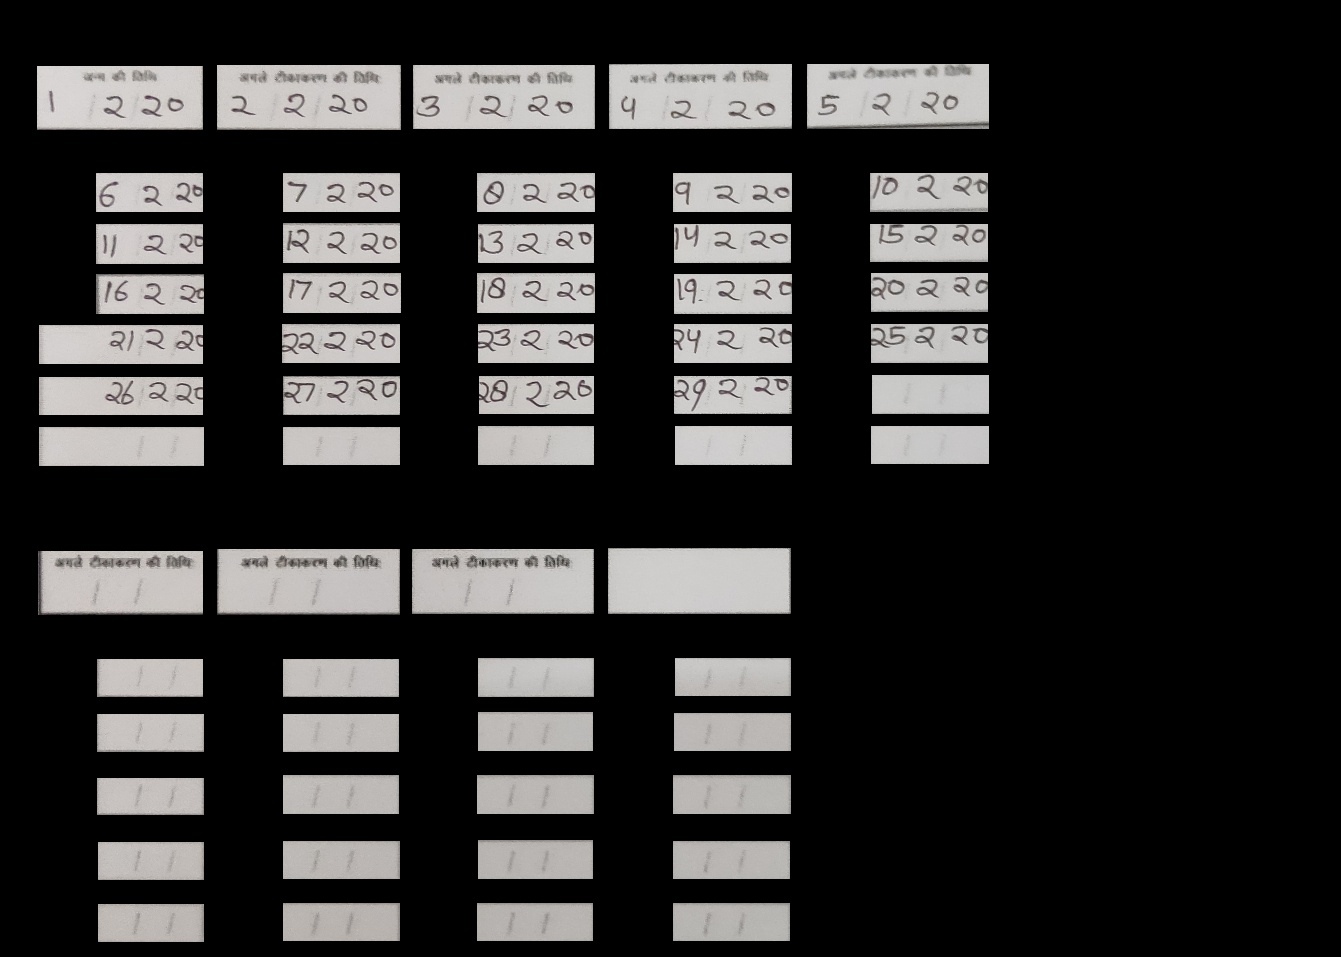
\includegraphics[scale=.25]{4/.report/_segmented/_mask/p2.jpg}
      \caption{Printout2}
    \end{center}
    \endminipage
    \end{figure}
% -------------------------------------------------------
\pagebreak \\
\textbf{Masked}
    \begin{figure}[!htb]
    %
    \minipage{\textwidth}
    \begin{center}
      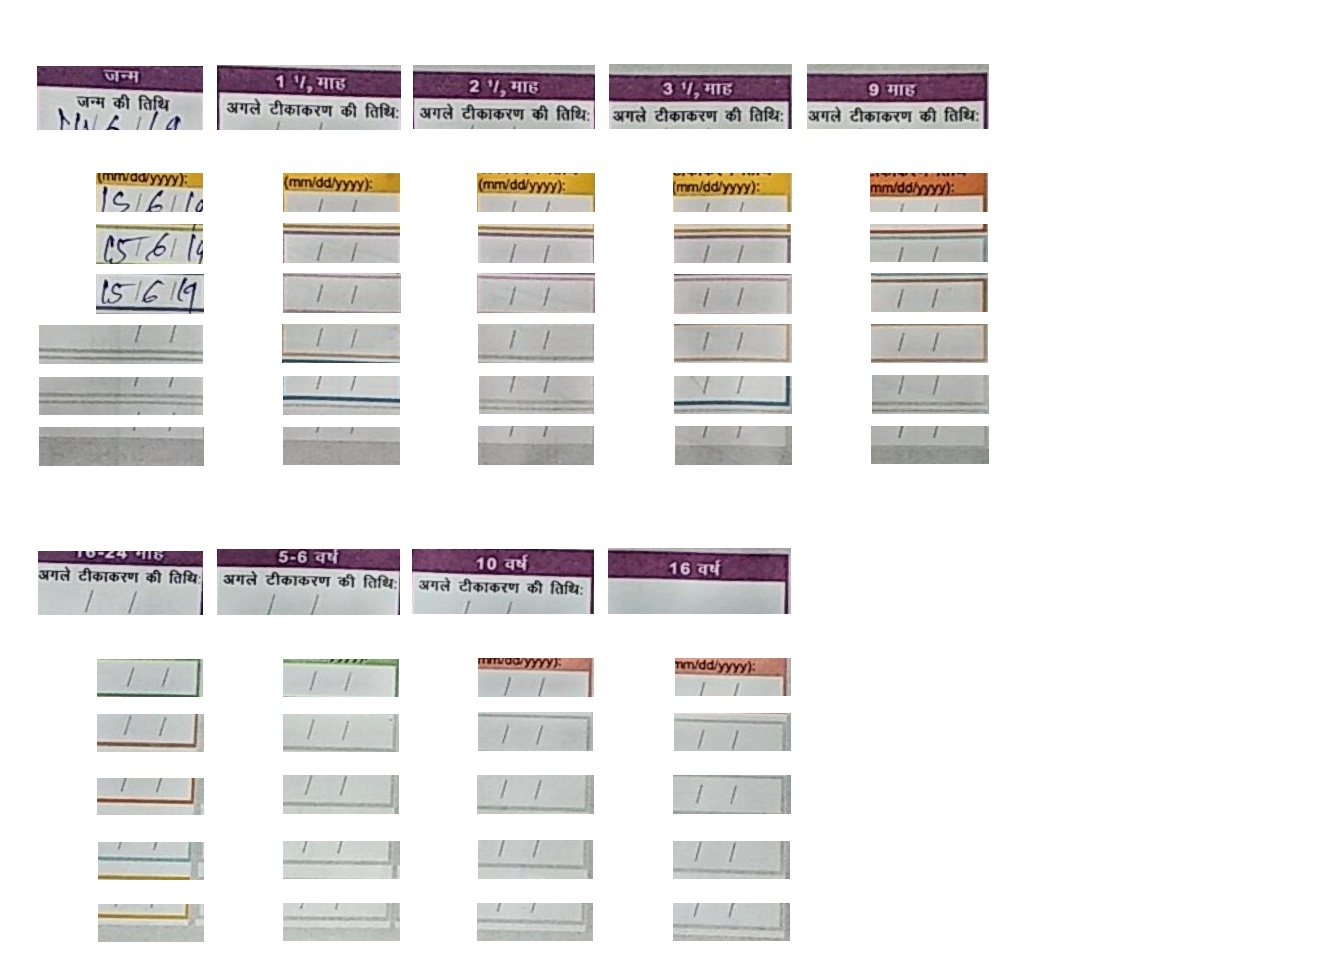
\includegraphics[scale=.25]{4/.report/_segmented/_mask/b1.jpg}
      \caption{Booklet1}
    \end{center}
    \endminipage
    \end{figure}
    \begin{figure}[!htb]
    %
    \minipage{\textwidth}
    \begin{center}
      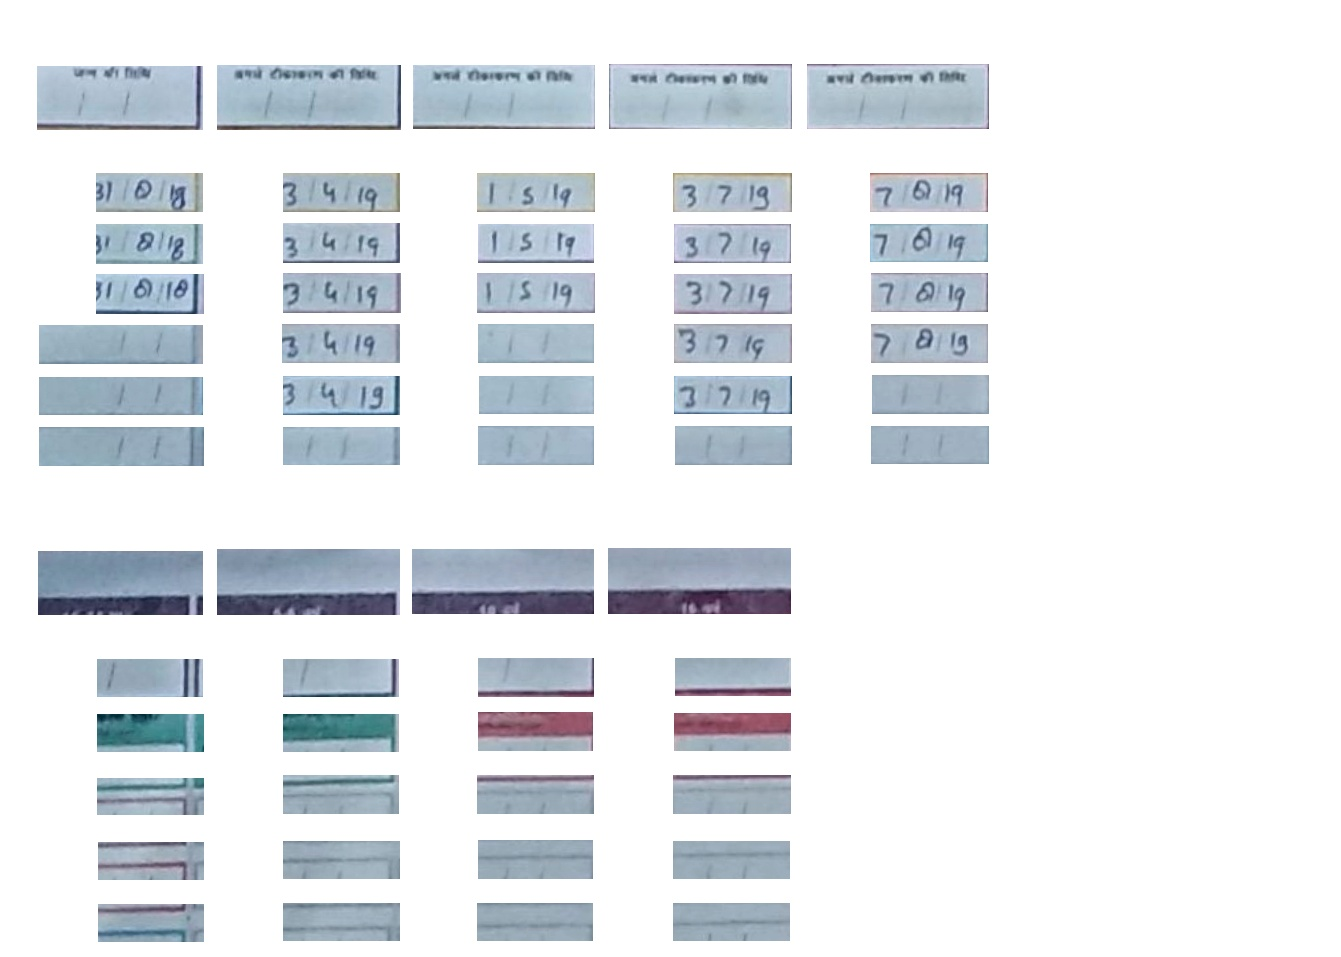
\includegraphics[scale=.25]{4/.report/_segmented/_mask/b2.jpg}
      \caption{Booklet2}
    \end{center}
    \endminipage
    \end{figure}
% ------------------------------------------------------- 
% ------------------------------------------------------- 
    \pagebreak
% -------------------------------------------------------
% Character Detection
    \subsection*{Character detection}
    Having segmented the image, using the latter approach (masking), it was fairly easy to do character detection using thresholding and then contouring the remaining characters.\\[1pt]
    Note: The thresholding was binary, after adaptive histogram-equlisationn was applied to the aligned image. This allowed for faster and easier detection.\\
    \textit{Bonus}: It was observed that median filtering the images led to removal of pre-printed slashes and thus they didn't appear in the detected character-set.\\
    The results, including the detected characters and thresholding results are presented further.\\
% -------------------------------------------------------
% \pagebreak \\
\textbf{Scanned1}
    \begin{figure}[!htb]
    %
    \minipage{\textwidth}
    \begin{center}
      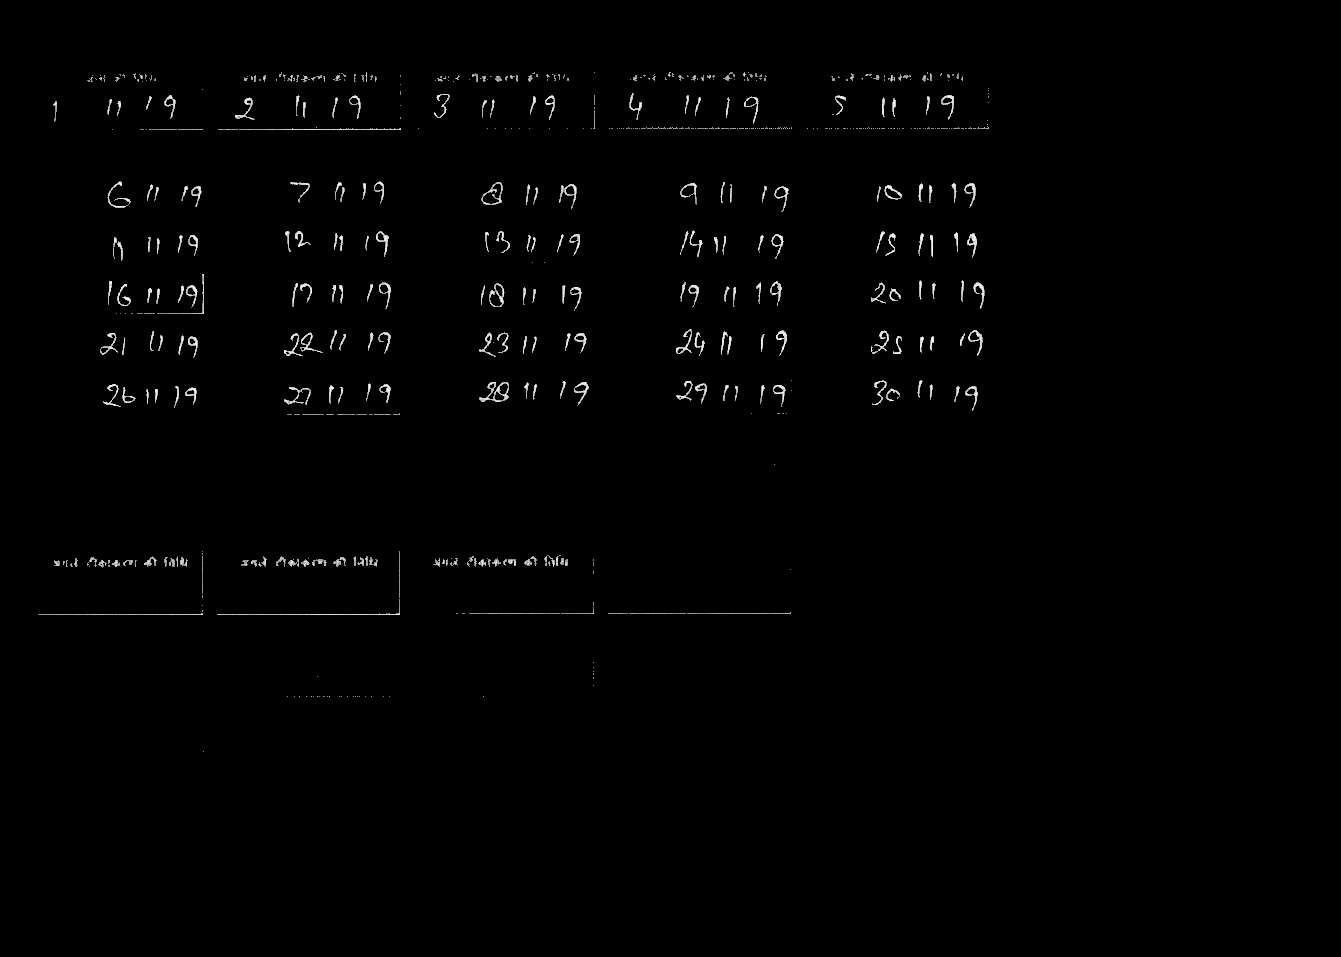
\includegraphics[scale=.15]{4/.report/_thresh/s1.jpg}
      \caption{Thresholded Image}
    \end{center}
    \endminipage
    \end{figure}
    \begin{figure}[!htb]
    %
    \minipage{\textwidth}
    \begin{center}
      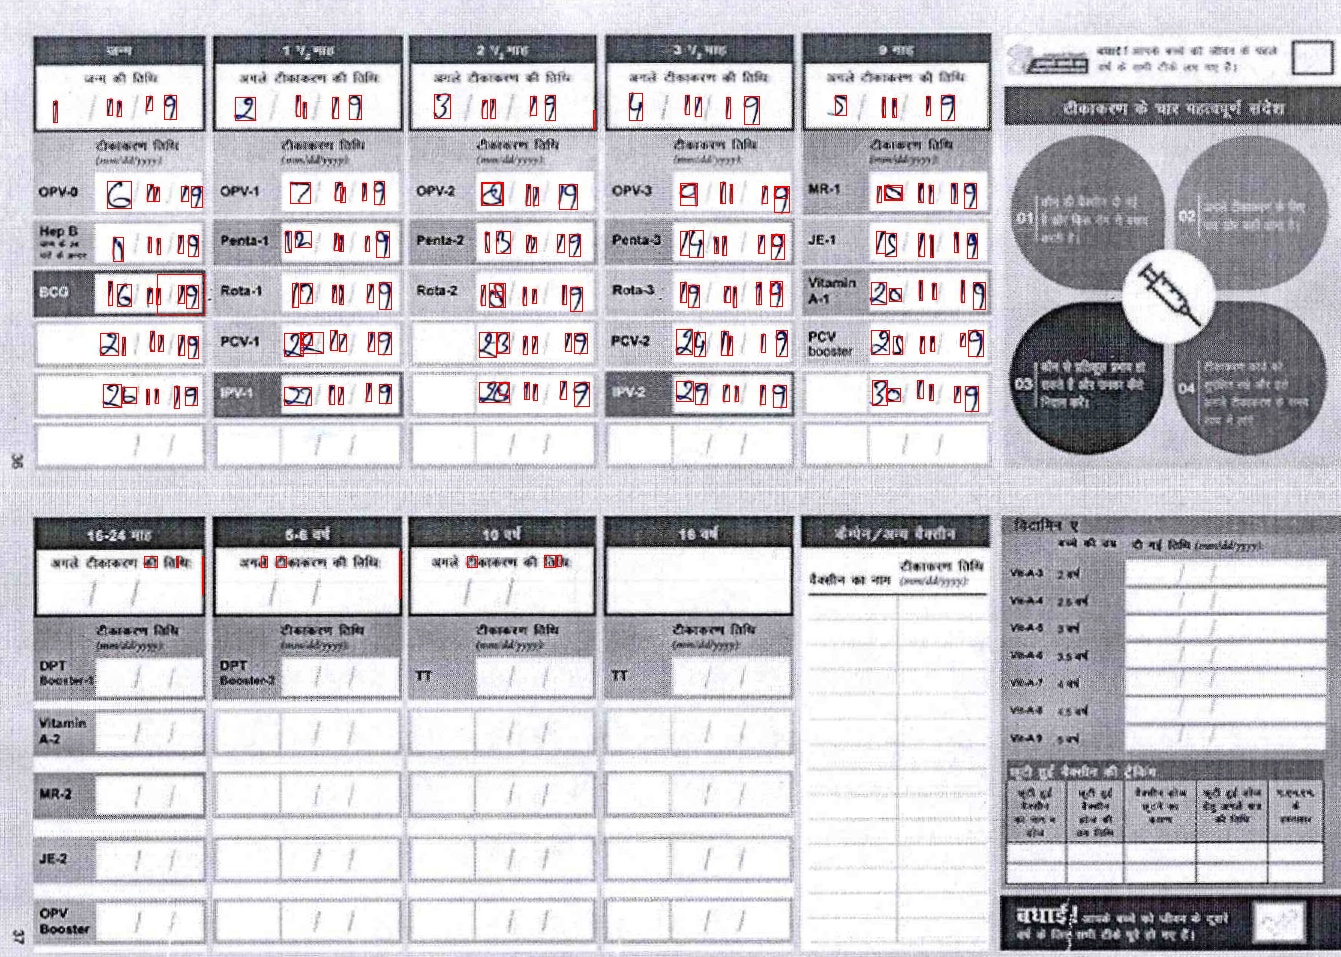
\includegraphics[scale=.15]{4/.report/_char/s1.jpg}
      \caption{Character Detection}
    \end{center}
    \endminipage
    \end{figure}
% -------------------------------------------------------
\pagebreak \\
\textbf{Scanned2}
    \begin{figure}[!htb]
    %
    \minipage{\textwidth}
    \begin{center}
      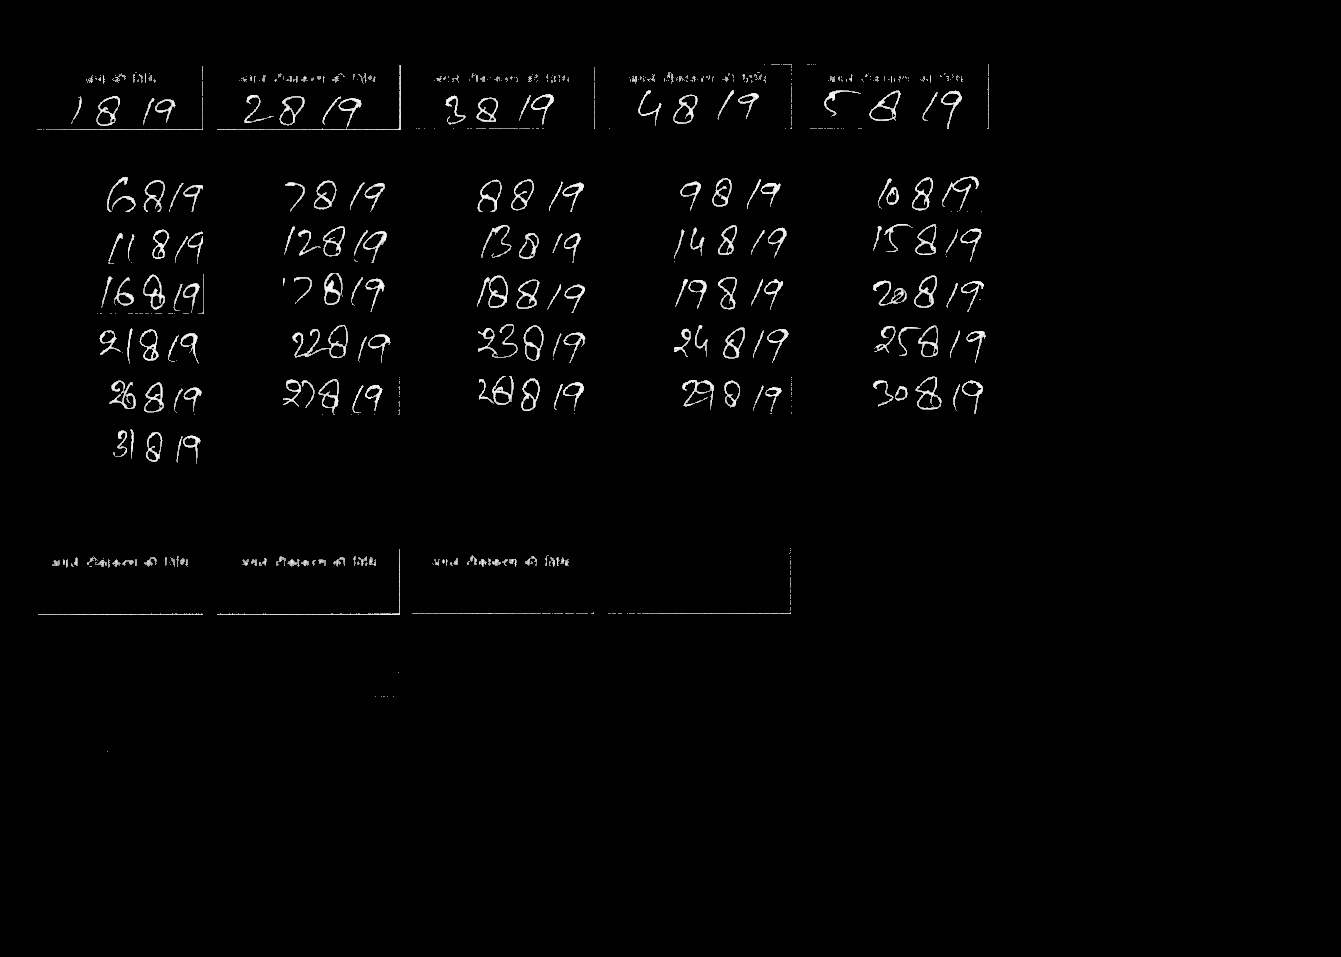
\includegraphics[scale=.25]{4/.report/_thresh/s2.jpg}
      \caption{Thresholded Image}
    \end{center}
    \endminipage
    \end{figure}
    \begin{figure}[!htb]
    %
    \minipage{\textwidth}
    \begin{center}
      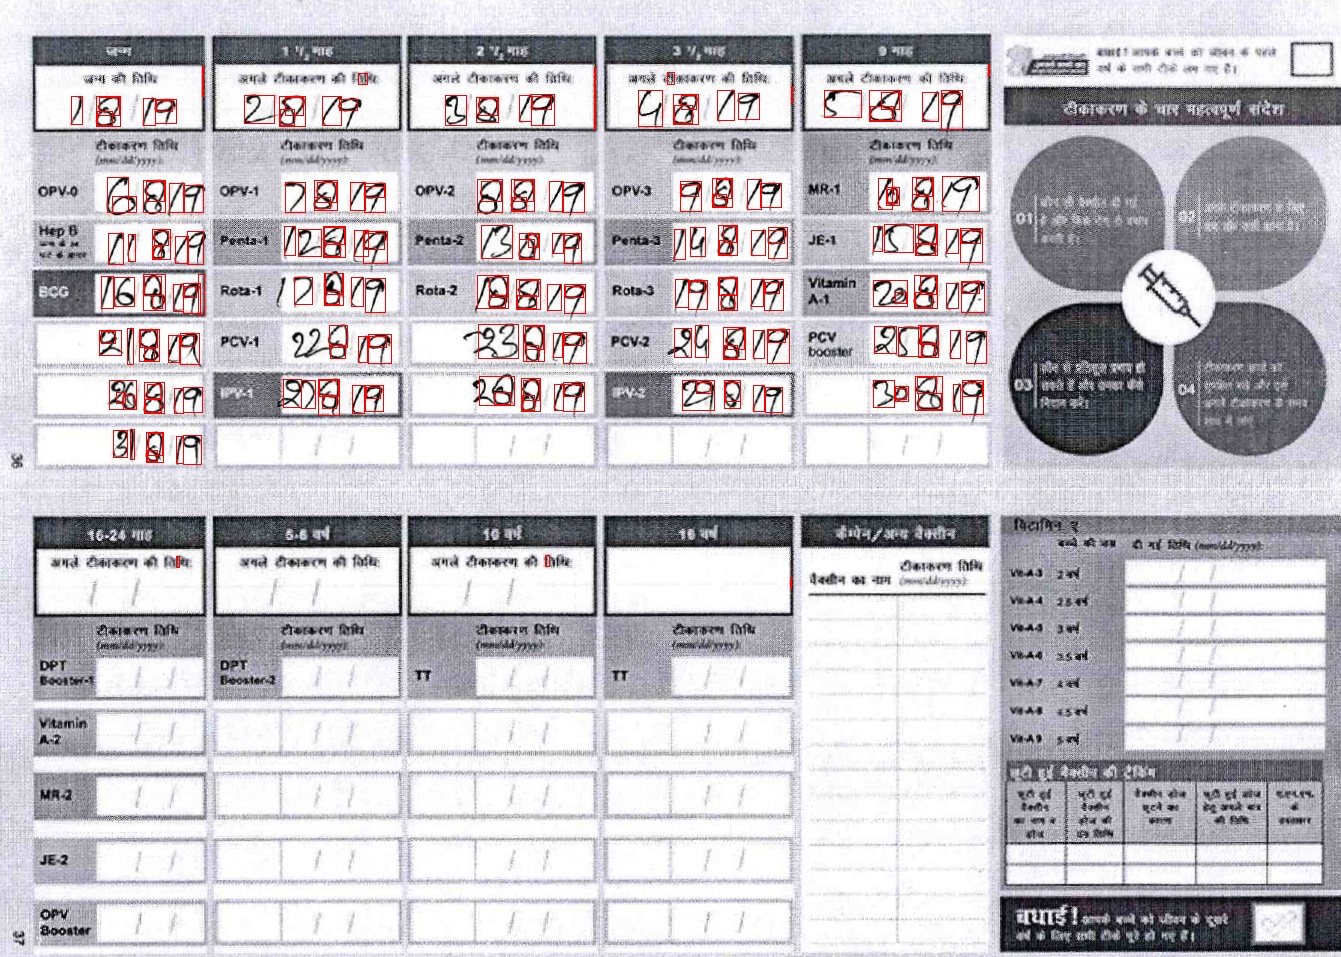
\includegraphics[scale=.25]{4/.report/_char/s2.jpg}
      \caption{Character Detection}
    \end{center}
    \endminipage
    \end{figure}
% -------------------------------------------------------
\pagebreak \\
\textbf{Printout1}
    \begin{figure}[!htb]
    %
    \minipage{\textwidth}
    \begin{center}
      \includegraphics[scale=.25]{4/.report/_thresh/p1.jpg}
      \caption{Thresholded Image}
    \end{center}
    \endminipage
    \end{figure}
    \begin{figure}[!htb]
    %
    \minipage{\textwidth}
    \begin{center}
      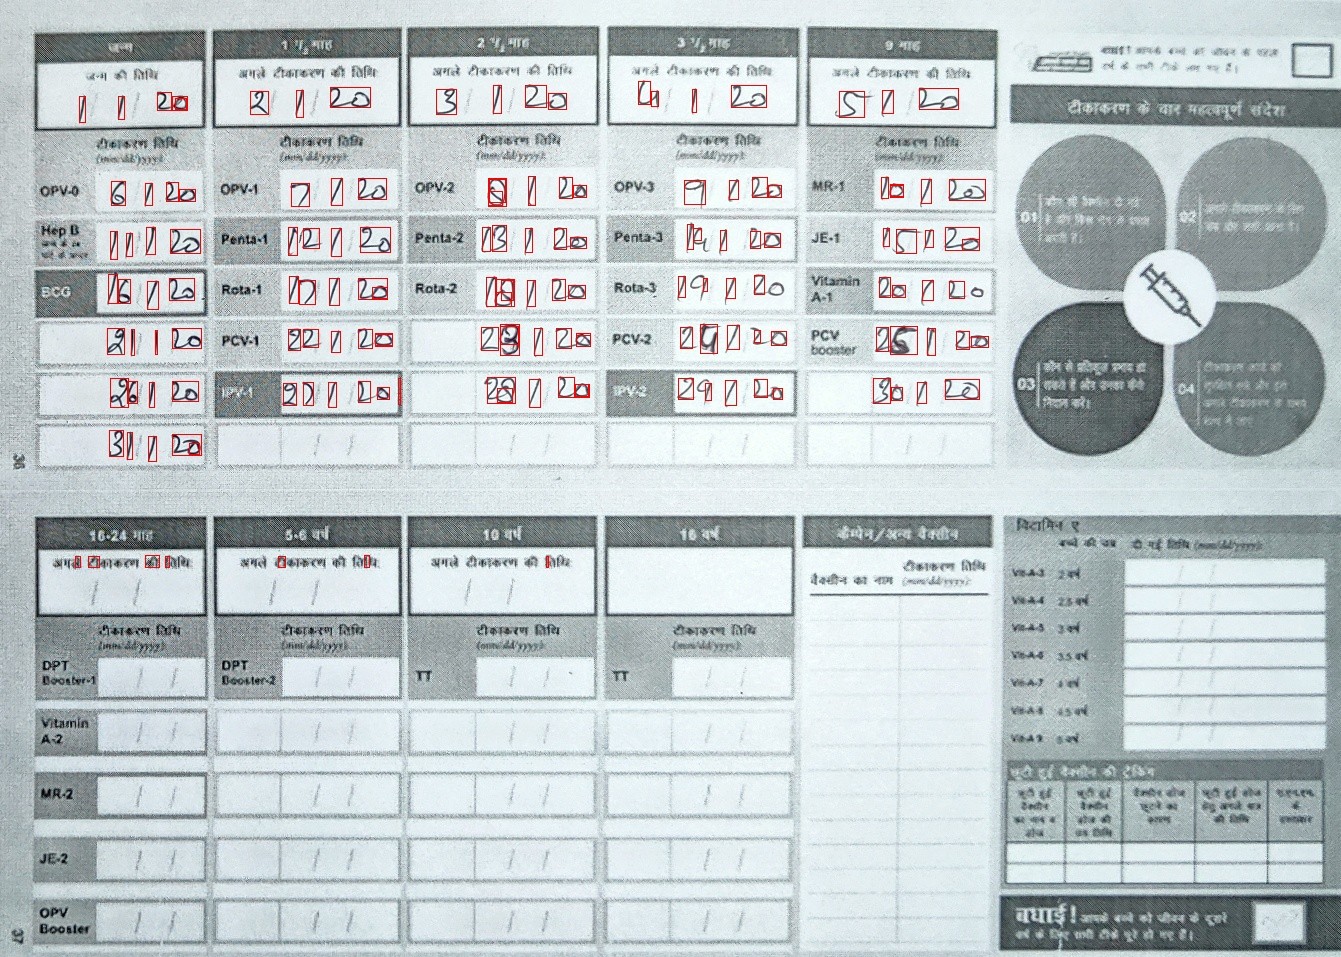
\includegraphics[scale=.25]{4/.report/_char/p1.jpg}
      \caption{Character Detection}
    \end{center}
    \endminipage
    \end{figure}
% -------------------------------------------------------
\pagebreak \\
\textbf{Printout2}
    \begin{figure}[!htb]
    %
    \minipage{\textwidth}
    \begin{center}
      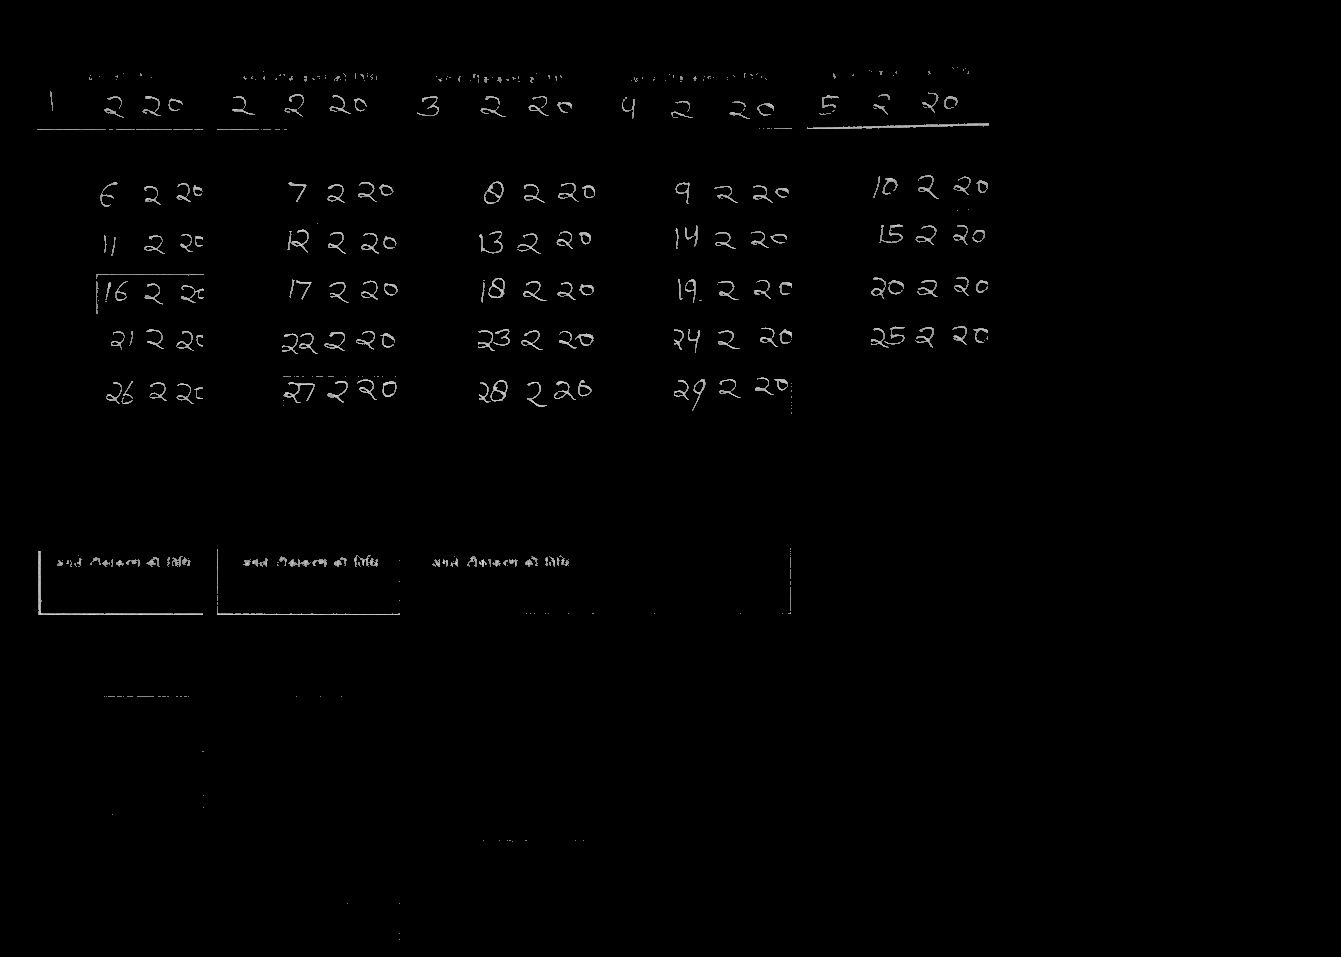
\includegraphics[scale=.25]{4/.report/_thresh/p2.jpg}
      \caption{Thresholded Image}
    \end{center}
    \endminipage
    \end{figure}
    \begin{figure}[!htb]
    %
    \minipage{\textwidth}
    \begin{center}
      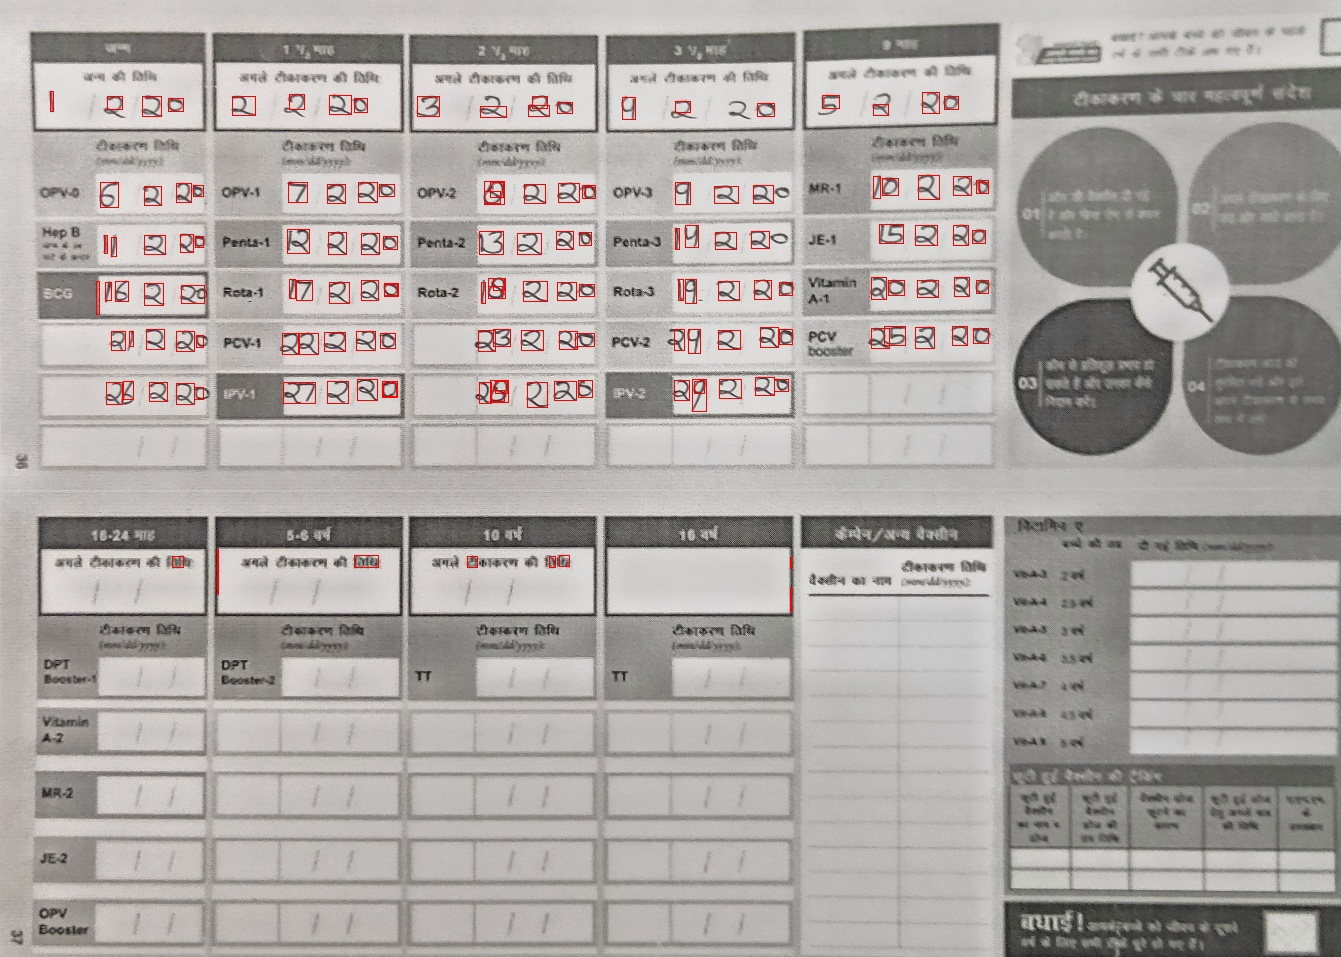
\includegraphics[scale=.25]{4/.report/_char/p2.jpg}
      \caption{Character Detection}
    \end{center}
    \endminipage
    \end{figure}
% -------------------------------------------------------
\pagebreak \\
\textbf{Booklet1}
    \begin{figure}[!htb]
    %
    \minipage{\textwidth}
    \begin{center}
      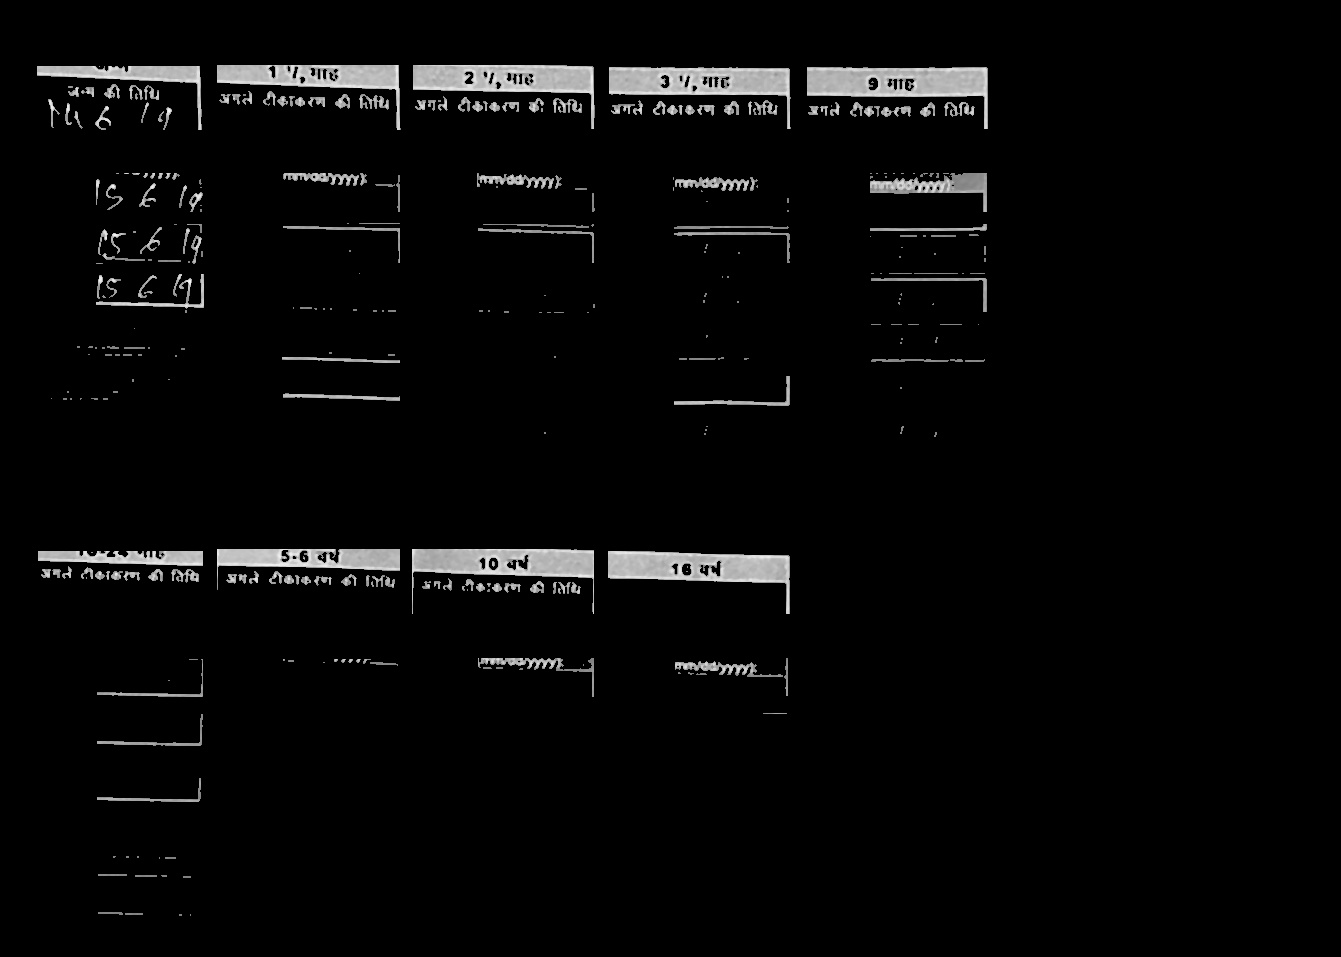
\includegraphics[scale=.25]{4/.report/_thresh/b1.jpg}
      \caption{Thresholded Image}
    \end{center}
    \endminipage
    \end{figure}
    \begin{figure}[!htb]
    %
    \minipage{\textwidth}
    \begin{center}
      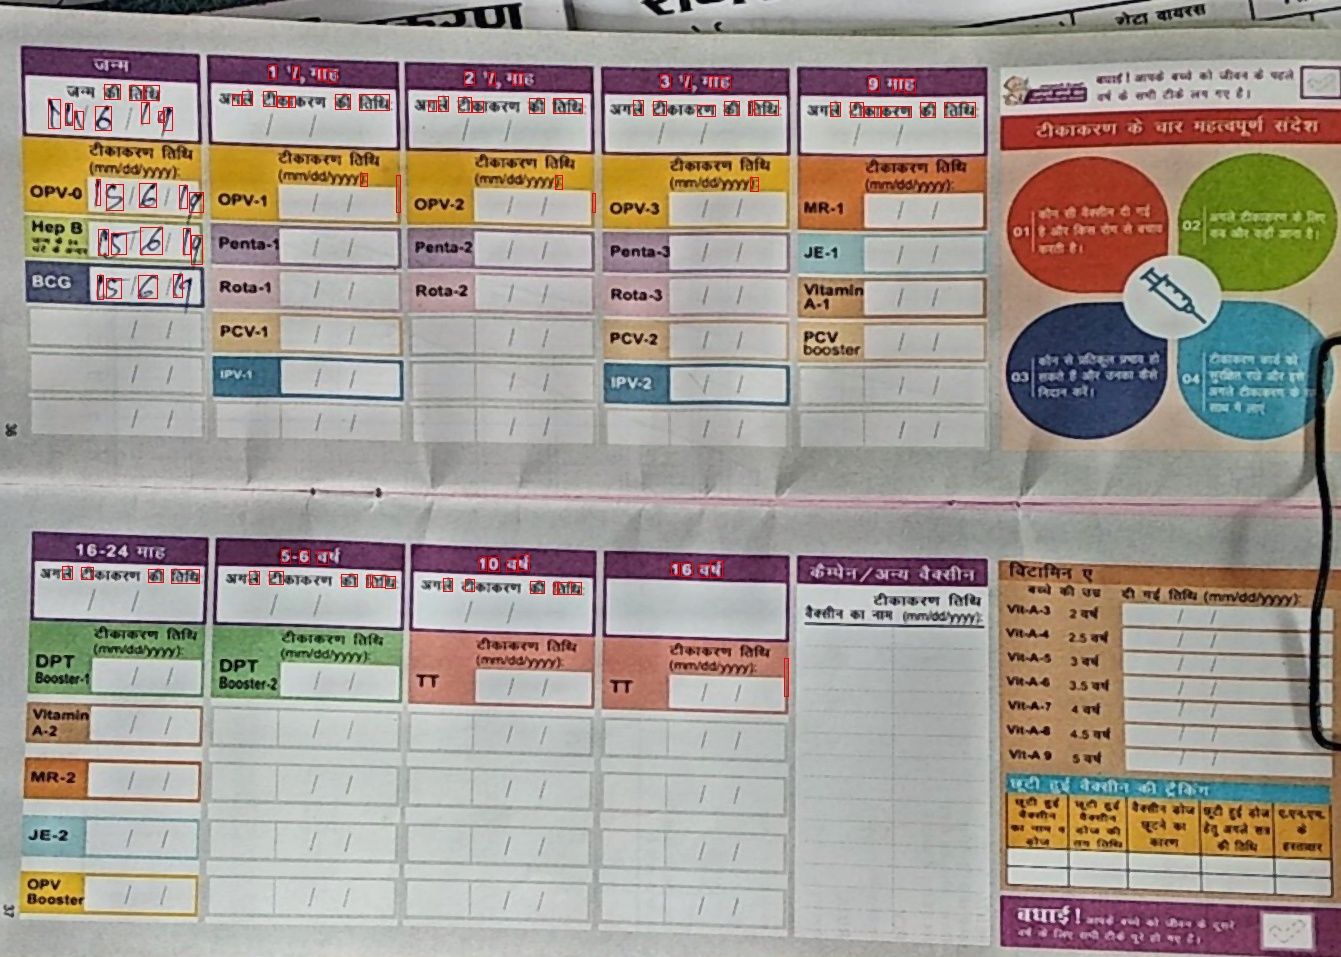
\includegraphics[scale=.25]{4/.report/_char/b1.jpg}
      \caption{Character Detection}
    \end{center}
    \endminipage
    \end{figure}
% -------------------------------------------------------
\pagebreak \\
\textbf{Booklet2}
    \begin{figure}[!htb]
    %
    \minipage{\textwidth}
    \begin{center}
      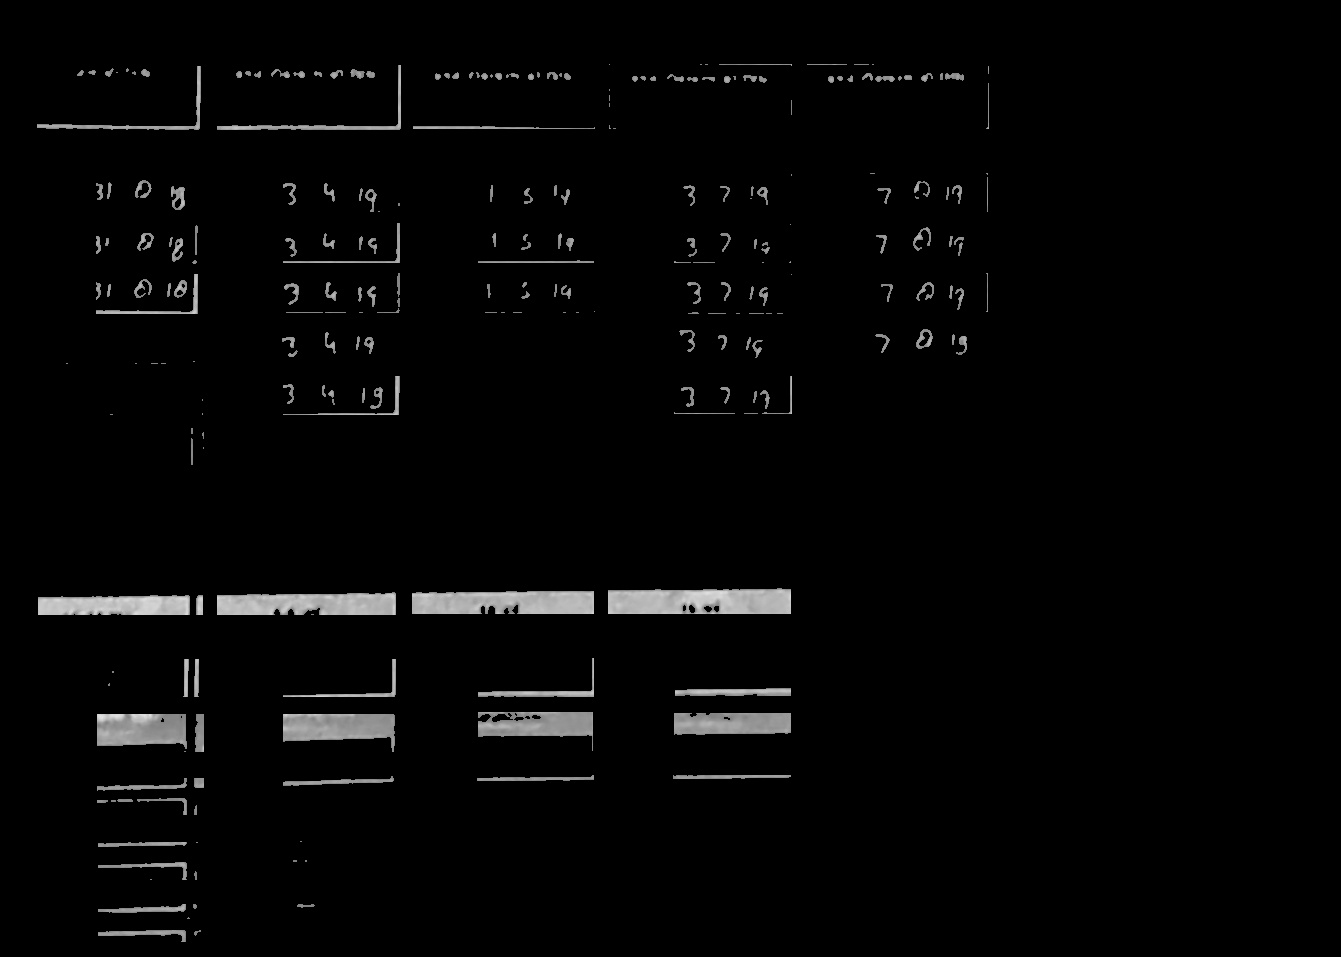
\includegraphics[scale=.25]{4/.report/_thresh/b2.jpg}
      \caption{Thresholded Image}
    \end{center}
    \endminipage
    \end{figure}
    \begin{figure}[!htb]
    %
    \minipage{\textwidth}
    \begin{center}
      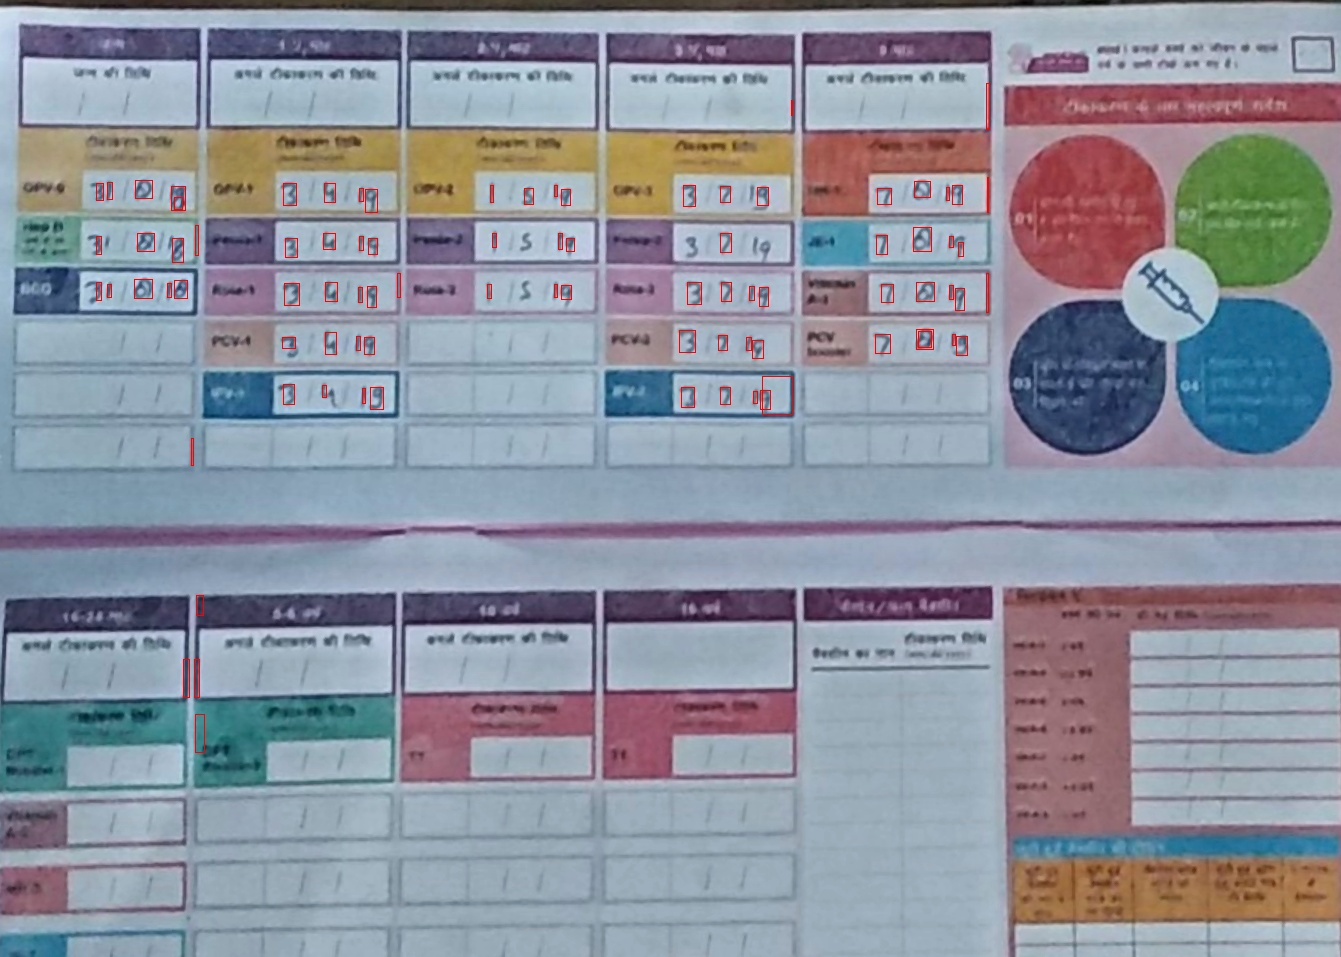
\includegraphics[scale=.25]{4/.report/_char/b2.jpg}
      \caption{Character Detection}
    \end{center}
    \endminipage
    \end{figure}
%--------------------------------------------- 
\pagebreak
%---------------------------------------------
% Summary
\subsection*{Summary}
    This assignment was very interesting, and I learnt a lot of new things.
    I really liked the idea of making this assignment open ended. As a direct practical application, we were very motivated to try all the possible things out and see how actually all methods we know of go around. \\
    What was discussed in class was very helpful. \\
    Thanks and Regards\\
    Rajbir
\end{document}